%-------------------------------------------------------------------------
%-------------------------------------------------------------------------
%-------------------------------------------------------------------------

\chapter[Field Study\texorpdfstring{:\\ Overview: The Design, Adoption, and Analysis of a Visual Document Mining Tool For Investigative Journalists}{}]{Field Study\texorpdfstring{:\\ \large{Overview: The Design, Adoption, and Analysis of a Visual Document Mining Tool For Investigative Journalists}}{}}
\label{ch:overview}



%-------------------------------------------------------------------------
%-------------------------------------------------------------------------
%-------------------------------------------------------------------------

\begin{epigraph}
    \emph{``The Street finds its own uses for things - uses the manufacturers never imagined.''} ---~William Gibson in ``Rocket Radio'' (\emph{Rolling Stone}, June 15, 1989)
\end{epigraph}

\footnote{This chapter is a slightly modified version of our paper {\it Overview: The Design, Adoption, and Analysis of a Visual Document Mining Tool For Investigative Journalists} by Matthew Brehmer, Stephen Ingram, Jonathan Stray, and Tamara Munzner; in IEEE Transactions on Visualization and Computer Graphics (Proceedings of InfoVis 2014), 20(12), p. 2271--2280~\cite{Brehmer2014}. \url{http://dx.doi.org/10.1109/TVCG.2014.2346431}. \autoref{overview:addendum} is a new addendum section that is unique to this dissertation. High-resolution versions of the figures in this chapter are available here: \url{http://cs.ubc.ca/labs/imager/tr/2014/Overview/}.}For an investigative journalist\index{journalism}, a large collection of documents\index{document data} obtained from a Freedom of Information Act (FOIA) request or a leak is both a blessing and a curse: such material may contain multiple newsworthy stories, but it can be difficult and time consuming to find relevant documents.
Standard text search is useful, but even if the search target is known it may not be possible to formulate an effective keyword search term.
In addition, summarization\index{{\tt summarize}} is an important non-search action.
We present {\it Overview}\footnote{Throughout this chapter, {\it Overview}\index{Overview (document mining tool)} is italicized to distinguish it from ``overview'', an overloaded term in the visualization literature.}, an application for the systematic analysis of large document collections\index{document data} based on document clustering, visualization, and tagging. 
This work contributes to the small set of studies which evaluate\index{evaluation} a visualization tool ``in the wild''\index{evaluation!in the wild}, and we report on six case studies\index{case study} where {\it Overview}\index{Overview (document mining tool)} was voluntarily used by self-initiated journalists\index{journalism} to produce published stories. 
We find that the frequently-used language of ``exploring''\index{{\tt explore}} a document collection\index{document data} is both too vague and too narrow to capture how journalists\index{journalism} actually used our application. 
Our iterative process, including multiple rounds of deployment and observations of real world usage, led to a much more specific classification of tasks\index{task}. 
We analyze and justify the visual encoding\index{visual encoding} and interaction\index{interaction} design choices used in {\it Overview}'s\index{Overview (document mining tool)} design with respect to our final task abstractions\index{task!task abstraction}, and propose transferable lessons for visualization design methodology.

%-------------------------------------------------------------------------
%-------------------------------------------------------------------------

\section{Motivation}
\label{overview:introduction}

%-------------------------------------------------------------------------
%-------------------------------------------------------------------------

\ac{FOIA} requests, leaks, government transparency initiatives, or other disclosures can result in thousands or millions of pages of potentially newsworthy material.
Investigative journalists\index{journalism} must find the stories lurking in these massive document collections\index{document data}, but it is frequently impossible to read every document.
Standard text search can be used to {\tt locate}\index{{\tt locate}} documents containing particular terms, but not all information retrieval\index{information retrieval} problems can be expressed as word search queries, especially if the relevant information is unexpected or novel.
Journalists\index{journalism} may also be interested in patterns of text across many documents, which can reveal significant trends, categories, or themes.
We conjectured that this {\it document mining}\index{document mining} problem could be solved by a visualization tool built around clustering and tagging documents.
The path from this hypothesis to a tool that working journalists\index{journalism} would voluntarily use was a long one; we needed to refine both our understanding of the problem and the ways in which journalists\index{journalism} might want to solve it.

%-|-|-|-|-|-|-|-|-|-|-|-|-|-|-|-|-|-|-|-|-|-|-|-|-|-|-|-|-|-|-|-|-|-|-|-|-

\begin{figure}
	\centering
	\fbox{\includegraphics[width=0.975\textwidth]{figures/overview-v4-sideways.pdf}}
	\caption
	[
	    \textsl{Overview} is a multiple-view application intended for the systematic search, summarization, annotation, and reading of a large collection of text documents.
	]
	{
    	\textsl{Overview} is a multiple-view application intended for the systematic {\tt search}, {\tt summarization}, {\tt annotation}, and reading of a large collection of text documents, hierarchically clustered based on content similarity and visualized as a tree (left). 
    	Pictured: a collection of White House email messages concerning drilling in the Gulf of Mexico prior to the 2010 Deepwater Horizon oil spill. 
	}
	\centering
	\label{overview:fig:overview-v4-teaser}
\end{figure}

%-|-|-|-|-|-|-|-|-|-|-|-|-|-|-|-|-|-|-|-|-|-|-|-|-|-|-|-|-|-|-|-|-|-|-|-|-

This chapter reports on the design, adoption\index{adoption}, and analysis of {\it Overview}\footnote{\url{https://www.overviewdocs.com/}}, an application developed by co-author Jonathan Stray in collaboration with our research group over several years.
{\it Overview}\index{Overview (document mining tool)}, shown in \autoref{overview:fig:overview-v4-teaser}, visualizes a document collection\index{document data} as a tree\index{visual encoding!tree} where nodes represent clusters of similar documents; a person can {\tt navigate}\index{{\tt navigate}} this tree\index{visual encoding!tree}, {\tt identify}\index{{\tt identify}} clusters, read individual documents, and {\tt annotate}\index{{\tt annotate}} documents with meaningful tags.
A timeline illustrating {\it Overview}'s\index{Overview (document mining tool)} development, deployment, and adoption\index{adoption} phases is shown in \autoref{overview:fig:timeline}.
Beginning with an initial use case, we developed a research prototype ({\it v1}), a publicly available cross-platform desktop application ({\it v2}), and finally a web-based application ({\it v3-v4}).
Ultimately, we succeeded in building a useful tool for journalists\index{journalism}:
we report on multiple case studies\index{case study} where {\it Overview}\index{Overview (document mining tool)} was adopted\index{adoption} for real investigations. 
Analysis of these cases revealed that journalists\index{journalism} often used the application in ways we did not anticipate, and we found that the often-used concept of ``exploring''\index{{\tt explore}} a document collection\index{document data} fails to capture the tasks\index{task} that journalists\index{journalism} actually perform.

%-|-|-|-|-|-|-|-|-|-|-|-|-|-|-|-|-|-|-|-|-|-|-|-|-|-|-|-|-|-|-|-|-|-|-|-|-

\begin{figure}
	\centering
	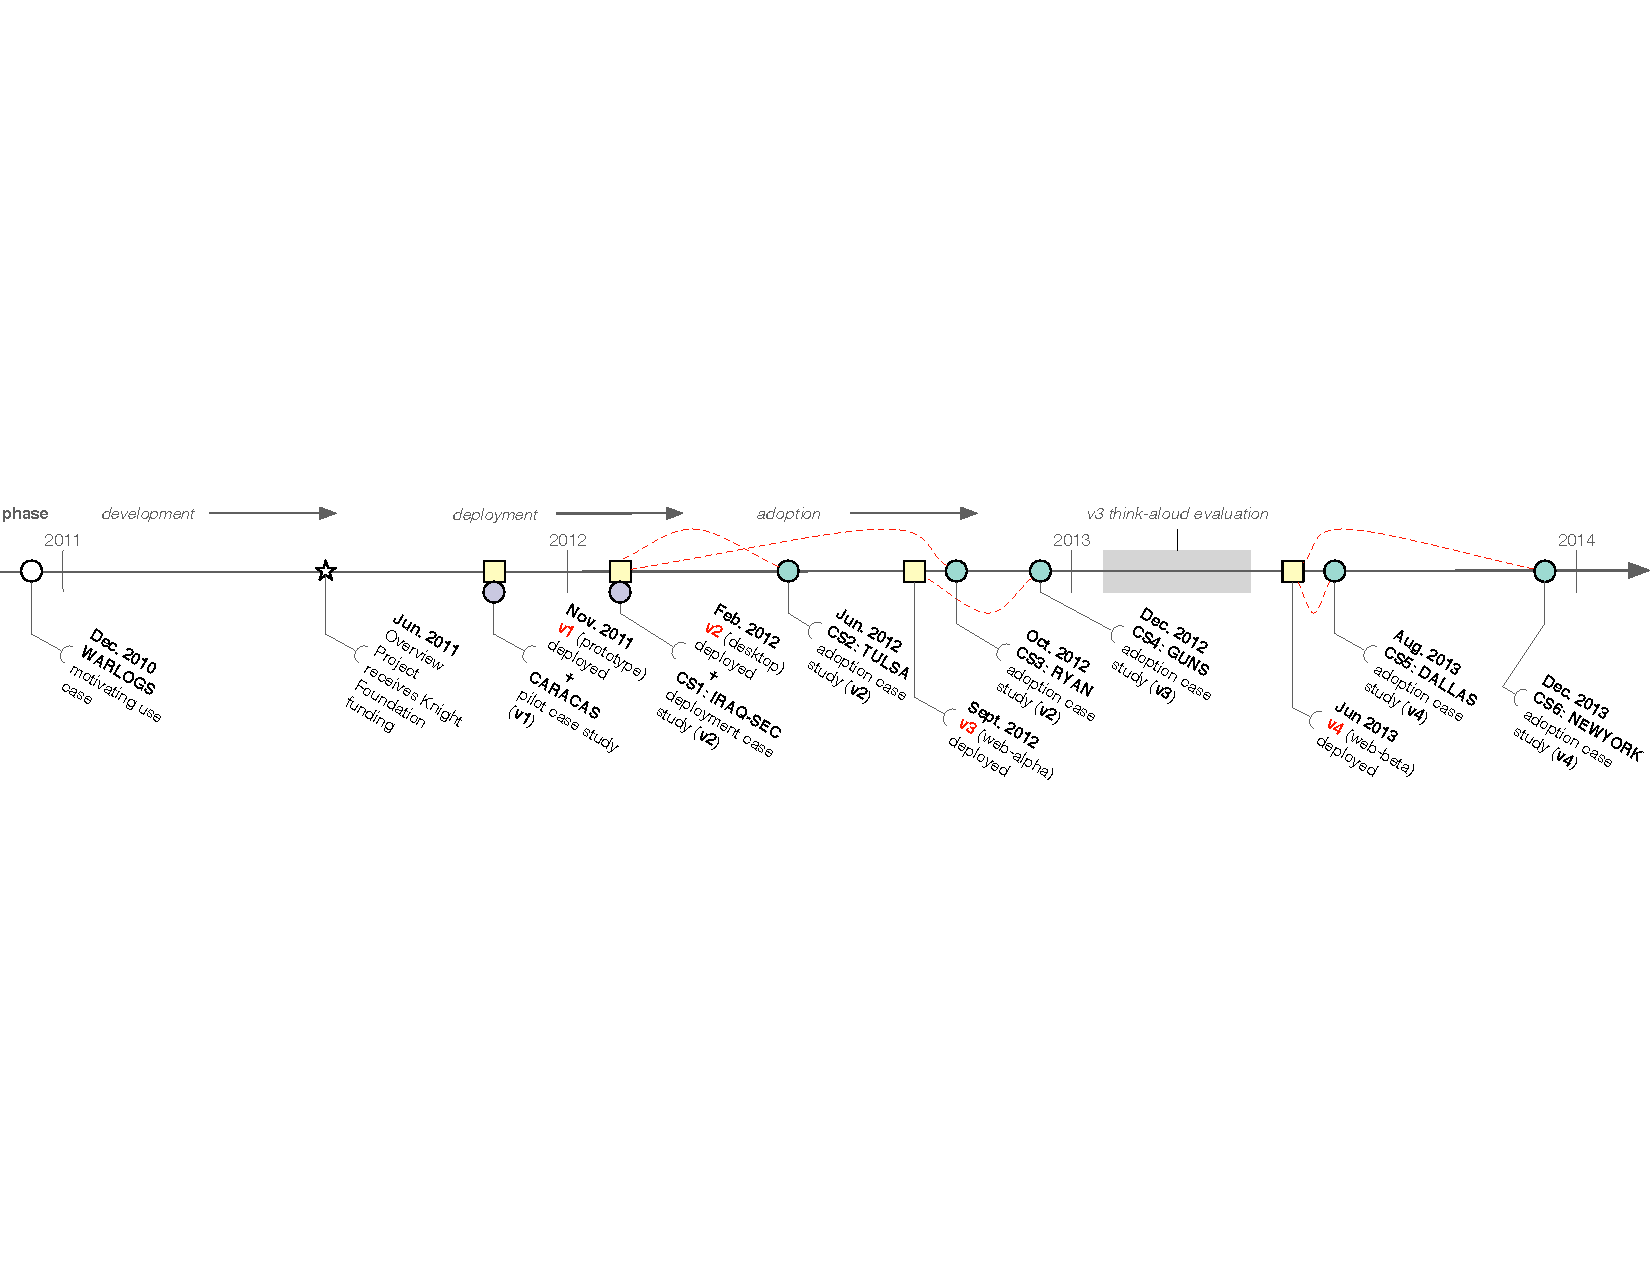
\includegraphics[width=0.975\textwidth]{figures/timeline.pdf}
	\caption
	[
	    A timeline of \textsl{Overview}'s development, deployment, and adoption phases.
	]
	{
	    A timeline of \textsl{Overview}'s development, deployment, and adoption phases: deployments are represented as yellow squares; deployment-phase case studies are represented as \raisebox{-.2\height}{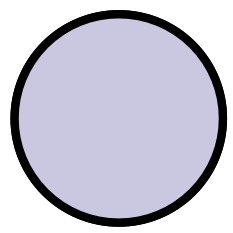
\includegraphics[width=0.015\textwidth, height=0.015\textwidth]{figures/deployment-case-study.png}} (purple circles), while adoption-phase case studies are represented as \raisebox{-.2\height}{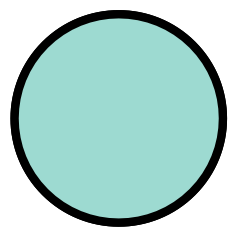
\includegraphics[width=0.015\textwidth, height=0.015\textwidth]{figures/adoption-case-study.png}} (turquoise circles).
	    The dotted red lines indicate which version of \textsl{Overview} was used in each case study.
	}
	\centering
	\label{overview:fig:timeline}
\end{figure}

%-|-|-|-|-|-|-|-|-|-|-|-|-|-|-|-|-|-|-|-|-|-|-|-|-|-|-|-|-|-|-|-|-|-|-|-|-

We frame this work as a visualization field study, one that took place during and after a process of iterative design addressing a particular domain problem, involving collaborators and people from that domain.
The contributions of this chapter include our classification of data\index{data abstraction} and task abstractions\index{task!task abstraction}, a description of its usage in real investigations spanning four deployments and six case studies\index{case study}, and a detailed analysis of the mapping from these abstractions\index{task!task abstraction} to visual encoding\index{visual encoding} and interaction\index{interaction} design choices.
This analysis led to important design revisions, based on a better understanding of {\it why}\index{{\tt why}} and {\it how}\index{{\tt how}} journalists\index{journalism} use {\it Overview}\index{Overview (document mining tool)}. 
From this experience we propose transferable lessons for visualization design methodology.

% The remainder of this chapter is organized as follows:
% We begin with a survey of related work in \autoref{overview:rw}.
% We then describe our initial use case in \autoref{overview:motivation}.
% The design of {\it Overview} is presented in \autoref{overview:overview}, which includes our initial task abstraction, {\it Overview}'s underlying data abstractions, and a description of its interface.
% In \autoref{overview:usage}, we report on real world usage of {\it Overview} by six journalists who used it for their own investigations; in five of these cases, the investigation resulted in a published story.
% Based on our observations of what these people did, we revisit our initial task abstraction and reflect upon the rationale for {\it Overview}'s visual encoding and interaction design choices in \autoref{overview:analysis}.
% Finally, in \autoref{overview:discussion}, we reflect on the methodological implications of our approach, and \autoref{overview:conclusion} summarizes our contributions.

%-------------------------------------------------------------------------
%-------------------------------------------------------------------------

\section{Related Work}
\label{overview:rw}

%-------------------------------------------------------------------------
%-------------------------------------------------------------------------

There have been a number of approaches and tools to support the analysis of document collections\index{document data}, spanning a range of data transformations and visual encodings\index{visual encoding}.  
We also review how these tools were evaluated\index{evaluation}.

\bstart{Topic model visualization}
One common approach to visualizing a document collection\index{document data} uses probabilistic topic models\index{topic models} inferred from the collection. 
These define topics as distributions of words and assign a distribution of topics per document. 
Both distributions are visualized directly in recent work by \citet{Chaney2012}, while other tools or techniques focus on the number of documents in each topic~\cite{Cui2011,Dou2013,Liu2012}, or use the topic assignments to compute the similarity between documents ~\cite{Chen2009,Eisenstein2012}. 
{\it Overview}\index{Overview (document mining tool)} does not use distribution-based topic models\index{topic models} but directly creates a hard hierarchical clustering\index{algorithms!clustering}, which is visually encoded as a tree\index{visual encoding!tree}.

\bstart{Documents as points}
Many visualization tools, including the first two versions of {\it Overview}\index{Overview (document mining tool)}, encode\index{{\tt encode}} individual documents as points in a scatterplot\index{visual encoding!scatterplot}. 
InfoSky~\cite{Granitzer2004} places points according to a pre-existing hierarchical arrangement\index{{\tt arrange}} of documents; in contrast, {\it Overview}\index{Overview (document mining tool)} is intended for document collections\index{document data} that do not have a pre-existing hierarchical structure\index{hierarchical data}. 
Other approaches begin with an unstructured document collection\index{document data} and place points based on document similarity metrics and \ac{DR}\index{dimensionality reduction (DR)} techniques, such as Leaksplorer~\cite{Leaksplorer}, PEx~\cite{Paulovich2007}, and EV~\cite{Chen2009}. 
{\it Overview v1-v2} included a similar scatterplot\index{visual encoding!scatterplot} which placed points by \ac{DR}\index{dimensionality reduction (DR)} through \ac{MDS}\index{dimensionality reduction (DR)!multi-dimensional scaling (MDS)}.
Finally, ForceSPIRE~\cite{Endert2012b} and TopicViz~\cite{Eisenstein2012} incorporate a scatterplot\index{visual encoding!scatterplot} where points corresponding to documents can be interactively placed according to one's own semantics or mental model, adaptively adjusting the underlying similarity metric used between document pairs.
In \autoref{overview:rationale}, we discuss in greater detail why a scatterplot\index{visual encoding!scatterplot} was omitted from later versions of {\it Overview}\index{Overview (document mining tool)}, and how tagging documents and clusters is an effective alternative to interactive placement.

\bstart{Documents as landscapes or clouds}
Document collections\index{document data} have also been encoded\index{{\tt encode}} as landscapes, three-dimensional visual encodings\index{visual encoding!scatterplot!3D scatterplot} of two- dimensional scatterplots\index{visual encoding!scatterplot} where height represents density, as in In-Spire~\cite{Hetzler2004} and recent work by \citet{Oesterling2011}.
However, empirical studies have shown that spatial landscapes are not well suited for encoding\index{{\tt encode}} inherently non-spatial data, and exhibit poor visual memory performance in comparison to two-dimensional scatterplots~\cite{Tory2009}\index{visual encoding!scatterplot}.

It is also possible to visualize a document collection\index{document data} by encoding\index{{\tt encode}} clusters of documents as interactive tag clouds\index{visual encoding!tag cloud}, as in Newdle~\cite{Liu2013}.
Once again, previous research has documented the perceptual drawbacks of tag clouds~\cite{Hearst2008}\index{visual encoding!tag cloud}.
By encoding\index{{\tt encode}} a document collection\index{document data} as a tree\index{visual encoding!tree}, {\it Overview}\index{Overview (document mining tool)} circumvents these issues.

\bstart{Documents as networks of entities}
Jigsaw's approach~\cite{Gorg2013,Kang2012} to document collection\index{document data} analysis differs from {\it Overview}\index{Overview (document mining tool)} in that it emphasizes the extraction of entities from documents, linking names, places, events, and dates, visualizing these relationships\index{network data}. 
The emphasis on entities is reflective of the domains in which Jigsaw is used, which include intelligence analysis\index{intelligence analysis}, law enforcement\index{law enforcement}, and academic research~\cite{Kang2012}.
Journalists\index{journalism} frequently start with barely-legible scanned documents which must first be converted to text through \ac{OCR}, greatly reducing the accuracy of standard entity extraction techniques.
As a flexible multiple-view application, Jigsaw also has a significant learning curve, and people have reported investing many months into learning how to use it~\cite{Kang2012}.
The journalists\index{journalism} we spoke to are accustomed to short deadlines and may only intermittently be working on a story involving a large document collection\index{document data}, so simplicity is a crucial requirement. 

\bstart{Documents as trees and rivers}
Like {\it Overview}\index{Overview (document mining tool)}, HierarchicalTopics~\cite{Dou2013} features a tree\index{visual encoding!tree} of document clusters\index{document data}, initially arranged\index{{\tt arrange}} by similar keywords.
It allows people to re-arrange\index{{\tt arrange}} the tree\index{visual encoding!tree} according to their own semantics, similar to how a person who uses ForceSPIRE can rearrange\index{{\tt arrange}} documents in a scatterplot~\cite{Endert2012b}\index{visual encoding!scatterplot}.
HierarchicalTopics~\cite{Dou2013} additionally allows people to track topic prevalence over time with a stacked area graph visual encoding in the style of a ThemeRiver~\cite{Havre2002}\index{visual encoding!stacked area graph}.
However, this approach requires temporal metadata that would be difficult to extract from the diverse document sources supported by {\it Overview}\index{Overview (document mining tool)}.

\bstart{Evaluating visual document mining tools}
Several of the aforementioned tools have been evaluated\index{evaluation} via controlled experiments and case studies\index{case study}.
Controlled experiments, such as those used to evaluate\index{evaluation} Newdle~\cite{Liu2013} or HierarchicalTopics~\cite{Dou2013}, often involve non-specialists conducting domain-agnostic tasks\index{task} specified by the researchers, who conjecture that they match with real world usage. 
Moreover, the documents used in these controlled experiments were collections of online news articles which are not appropriate test data for {\it Overview}\index{Overview (document mining tool)}, as professionally produced news articles are clean and homogeneous, unlike the diverse and messy documents obtained by our case study\index{case study} journalists\index{journalism}, which often contain little or no metadata; news articles are the output\index{{\tt output}} of the journalistic\index{journalism} document mining\index{document mining} process, not the input\index{{\tt input}}.

Most similar to our approach is a series of case studies\index{case study} of academic researchers, intelligence analysts\index{intelligence analysis}, and law enforcement\index{law enforcement} personnel who had adopted\index{adoption} Jigsaw~\cite{Kang2012}.
These case studies\index{case study} resulted in a better understanding of Jigsaw's utility in relation to the tasks\index{task} of people working in a specific application domain; like us, they identified similar barriers to adoption\index{adoption} and their results suggested new directions for design~\cite{Gorg2013,Gorg2014}.

%-------------------------------------------------------------------------
%-------------------------------------------------------------------------

\section{Initial Use Case}
\label{overview:motivation}

%-------------------------------------------------------------------------
%-------------------------------------------------------------------------

The {\it Overview}\index{Overview (document mining tool)} project began in December 2010, when journalist\index{journalism} and co-author Jonathan Stray visualized a subset (11,616 of 391,832) of the WikiLeaks Iraq War Logs~\cite{Stray2010}.
Journalists\index{journalism} had previously examined these documents by using text search to retrieve specific records and by visualizing the structured data fields such as time and location, but they had not attempted an analysis of the unstructured text of the reports.
In this initial use case, which we will refer to as {\sc warlogs}, documents were visualized as points placed according to a measure of similarity between documents and coloured according to pre-existing categorical labels, such as {\it ``friendly action''} and {\it ``criminal incident.''}  As shown in \autoref{overview:fig:warlogs}, this design revealed meaningful cluster structure that cross-cuts the colourings, showing that the pre-existing coarse categorization does not capture the whole story\footnote{The entire image is shown in \autoref{app:overview:initial-use-case}.}.

%-|-|-|-|-|-|-|-|-|-|-|-|-|-|-|-|-|-|-|-|-|-|-|-|-|-|-|-|-|-|-|-|-|-|-|-|-

\begin{figure}
	\centering
	\fbox{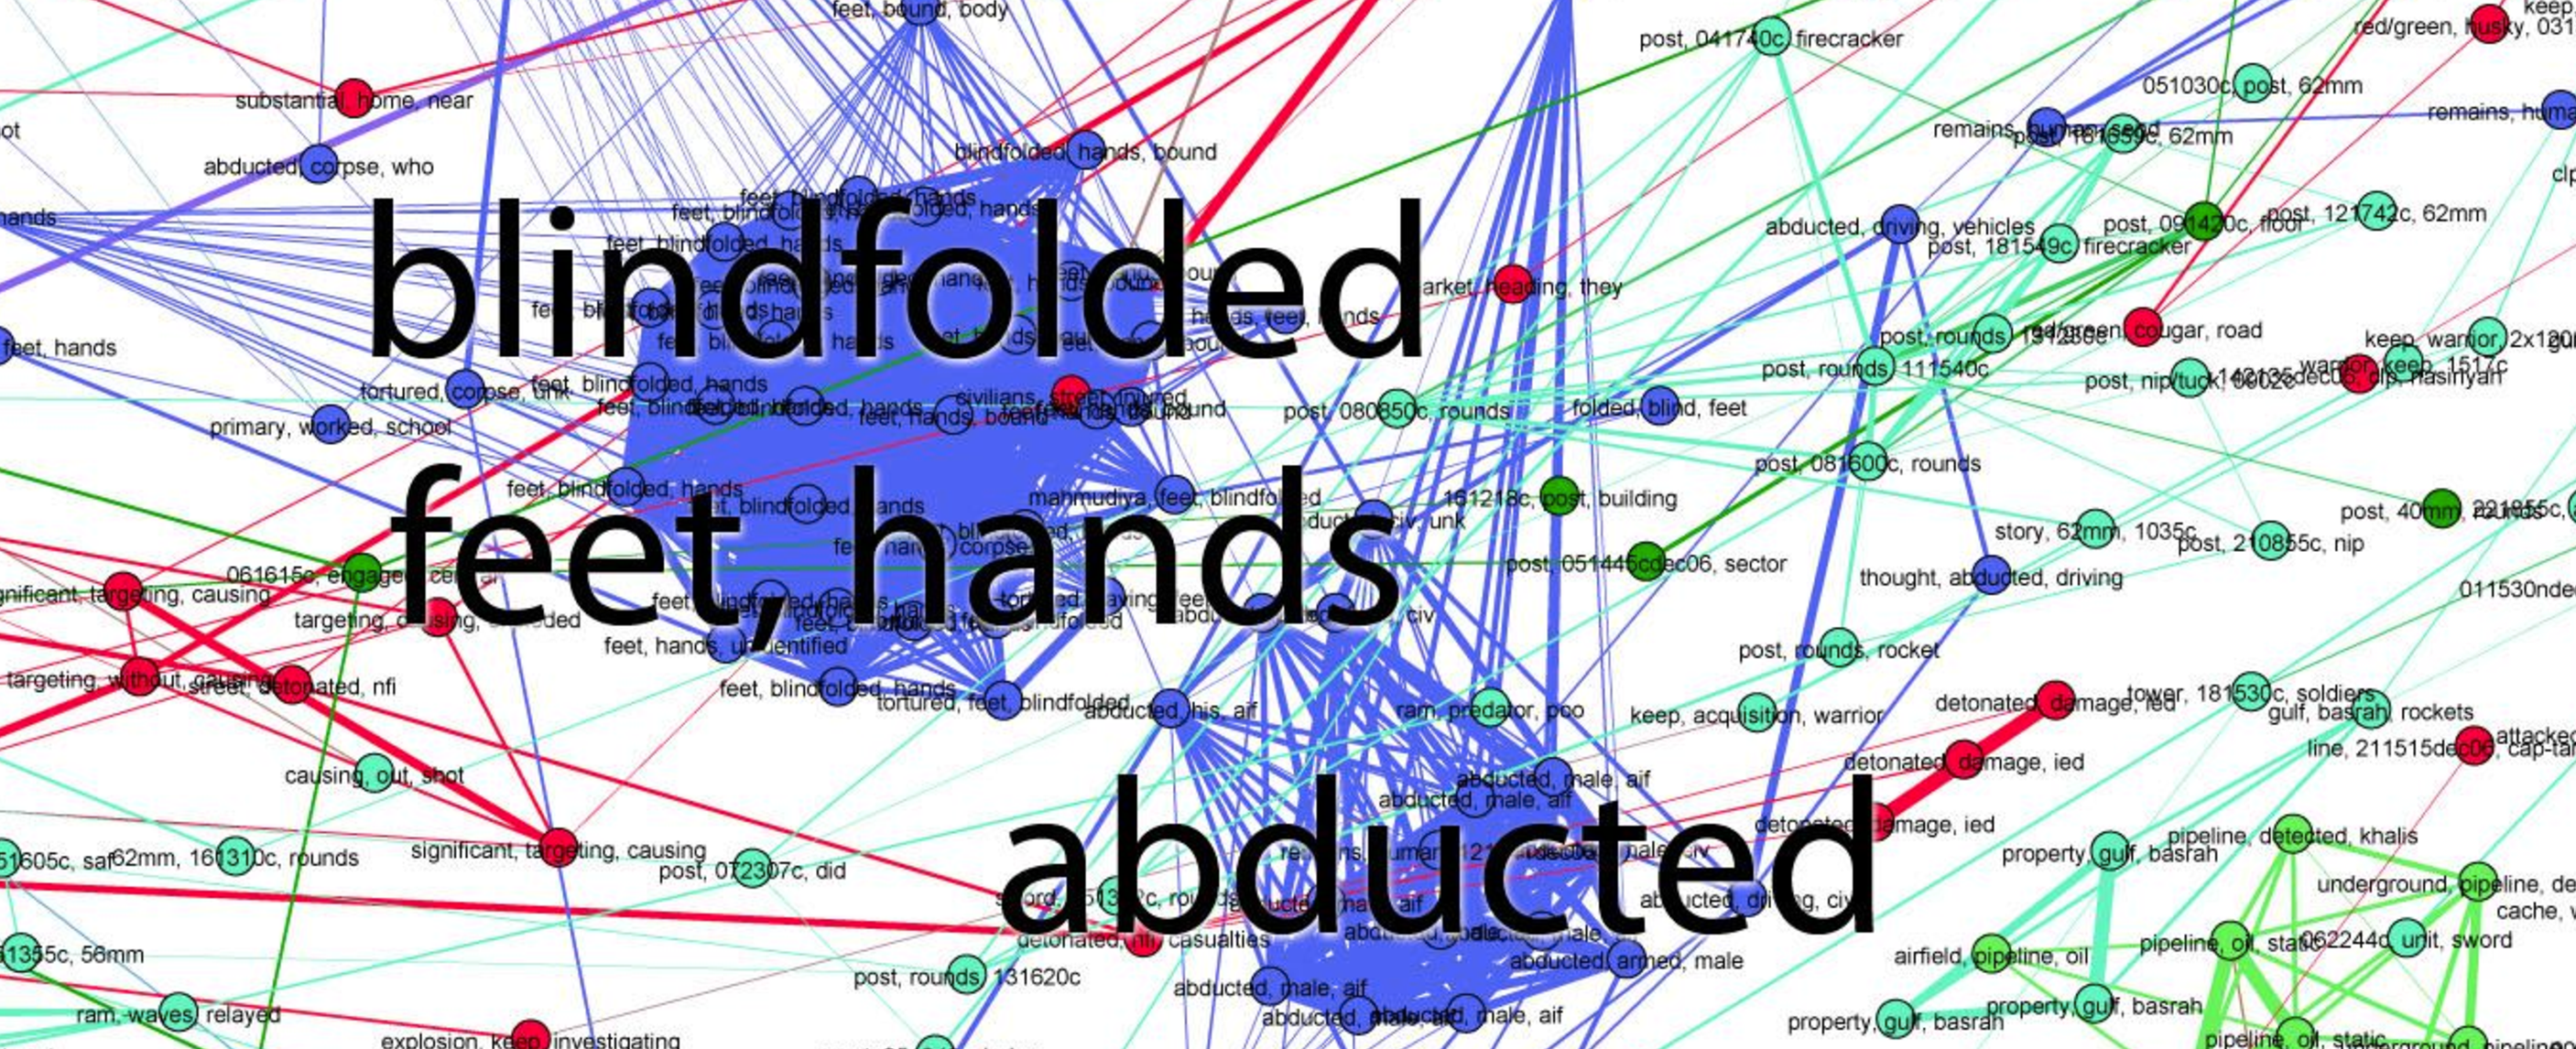
\includegraphics[width=0.975\textwidth]{figures/warlogs.pdf}}
	\caption
	[
	    Detail from \textsl{``A full-text visualization of the Iraq War Logs''}.
	]
	{
	    Detail from \textsl{``A full-text visualization of the Iraq War Logs''} ({\sc warlogs})~\cite{Stray2010}, in which distinct clusters of documents are visible; these documents pertain to ``criminal incidents'' during the Iraqi civil war involving abductions and blindfolding.
	}
	\centering
	\label{overview:fig:warlogs}
\end{figure}

%-|-|-|-|-|-|-|-|-|-|-|-|-|-|-|-|-|-|-|-|-|-|-|-|-|-|-|-|-|-|-|-|-|-|-|-|-

The {\sc warlogs} scatterplot\index{visual encoding!scatterplot} had serious limitations: it was not possible to interactively and systematically examine the contents of clusters of documents.
However, it demonstrated that visual cluster analysis could illuminate previously unknown and meaningful structure in a real world document collection\index{document data}, a conjecture that Stray had synthesized from his previous experience reporting on this collection of documents.
On the basis of this promising result, Stray collaborated with us to design an interactive visualization tool for document mining\index{document mining}.

%-------------------------------------------------------------------------
%-------------------------------------------------------------------------

\section{Design of Overview}
\label{overview:overview}

%-------------------------------------------------------------------------
%-------------------------------------------------------------------------

We now describe our initial task abstraction\index{task!task abstraction}, {\it Overview}'s\index{Overview (document mining tool)} underlying data abstractions, and the elements of its interface.

\bstart{Initial task abstraction}
During the development of {\it Overview v1-v2}, our task abstraction\index{task!task abstraction} was based on the {\sc warlogs} use case: journalists\index{journalism} would be motivated by the hypothesis that their document collection\index{document data} contained a semantically interesting cluster structure, and would require a means\index{task!means} for {\tt exploring}\index{{\tt explore}} that structure, drilling down into these clusters to examine the contained documents.
During this exploration\index{{\tt explore}}, they would need a way to keep track of what they had discovered, allowing them to revisit previously examined clusters and documents.

\bstart{Data abstractions}
Although {\it Overview}'s\index{Overview (document mining tool)} design has evolved over the course of four deployed versions, it continues to reflect several underlying data abstractions\index{data abstraction}.
{\it Overview}\index{Overview (document mining tool)} does not incorporate any novel text analysis\index{information retrieval} techniques; following a practice common in that domain, we convert each document to a vector of words weighted by the \ac{TF-IDF}\index{term frequency-inverse document frequency (TF-IDF)} formula, and compute similarity between documents using the cosine distance metric~\cite{Salton1988}.
We generate our document clusters\index{document data} by hierarchically clustering\index{algorithms!clustering} these distances and encoding\index{{\tt encode}} the result as a tree~\cite{Ingram2013,Ingram2012}\index{visual encoding!tree}.
Clusters are labeled with keywords extracted via \ac{TF-IDF}\index{term frequency-inverse document frequency (TF-IDF)} scores.

Multiple meaningful clusterings may exist for any collection of documents~\cite{Grimmer2011}; our particular distance metric and hierarchical clustering algorithm\index{algorithms!clustering} is but one possible choice.
Human-generated clusterings that leverage domain knowledge can complement automatic clusterings~\cite{Dou2013,Endert2012b}.
For these reasons, {\it Overview}\index{Overview (document mining tool)} allows for an arbitrary number of human-generated {\it tags} on each document, which can be assigned to individual documents or at the cluster level.
Tags allow people to keep track of what they have found and where they have looked so far.

%-|-|-|-|-|-|-|-|-|-|-|-|-|-|-|-|-|-|-|-|-|-|-|-|-|-|-|-|-|-|-|-|-|-|-|-|-

\begin{figure}
	\centering
	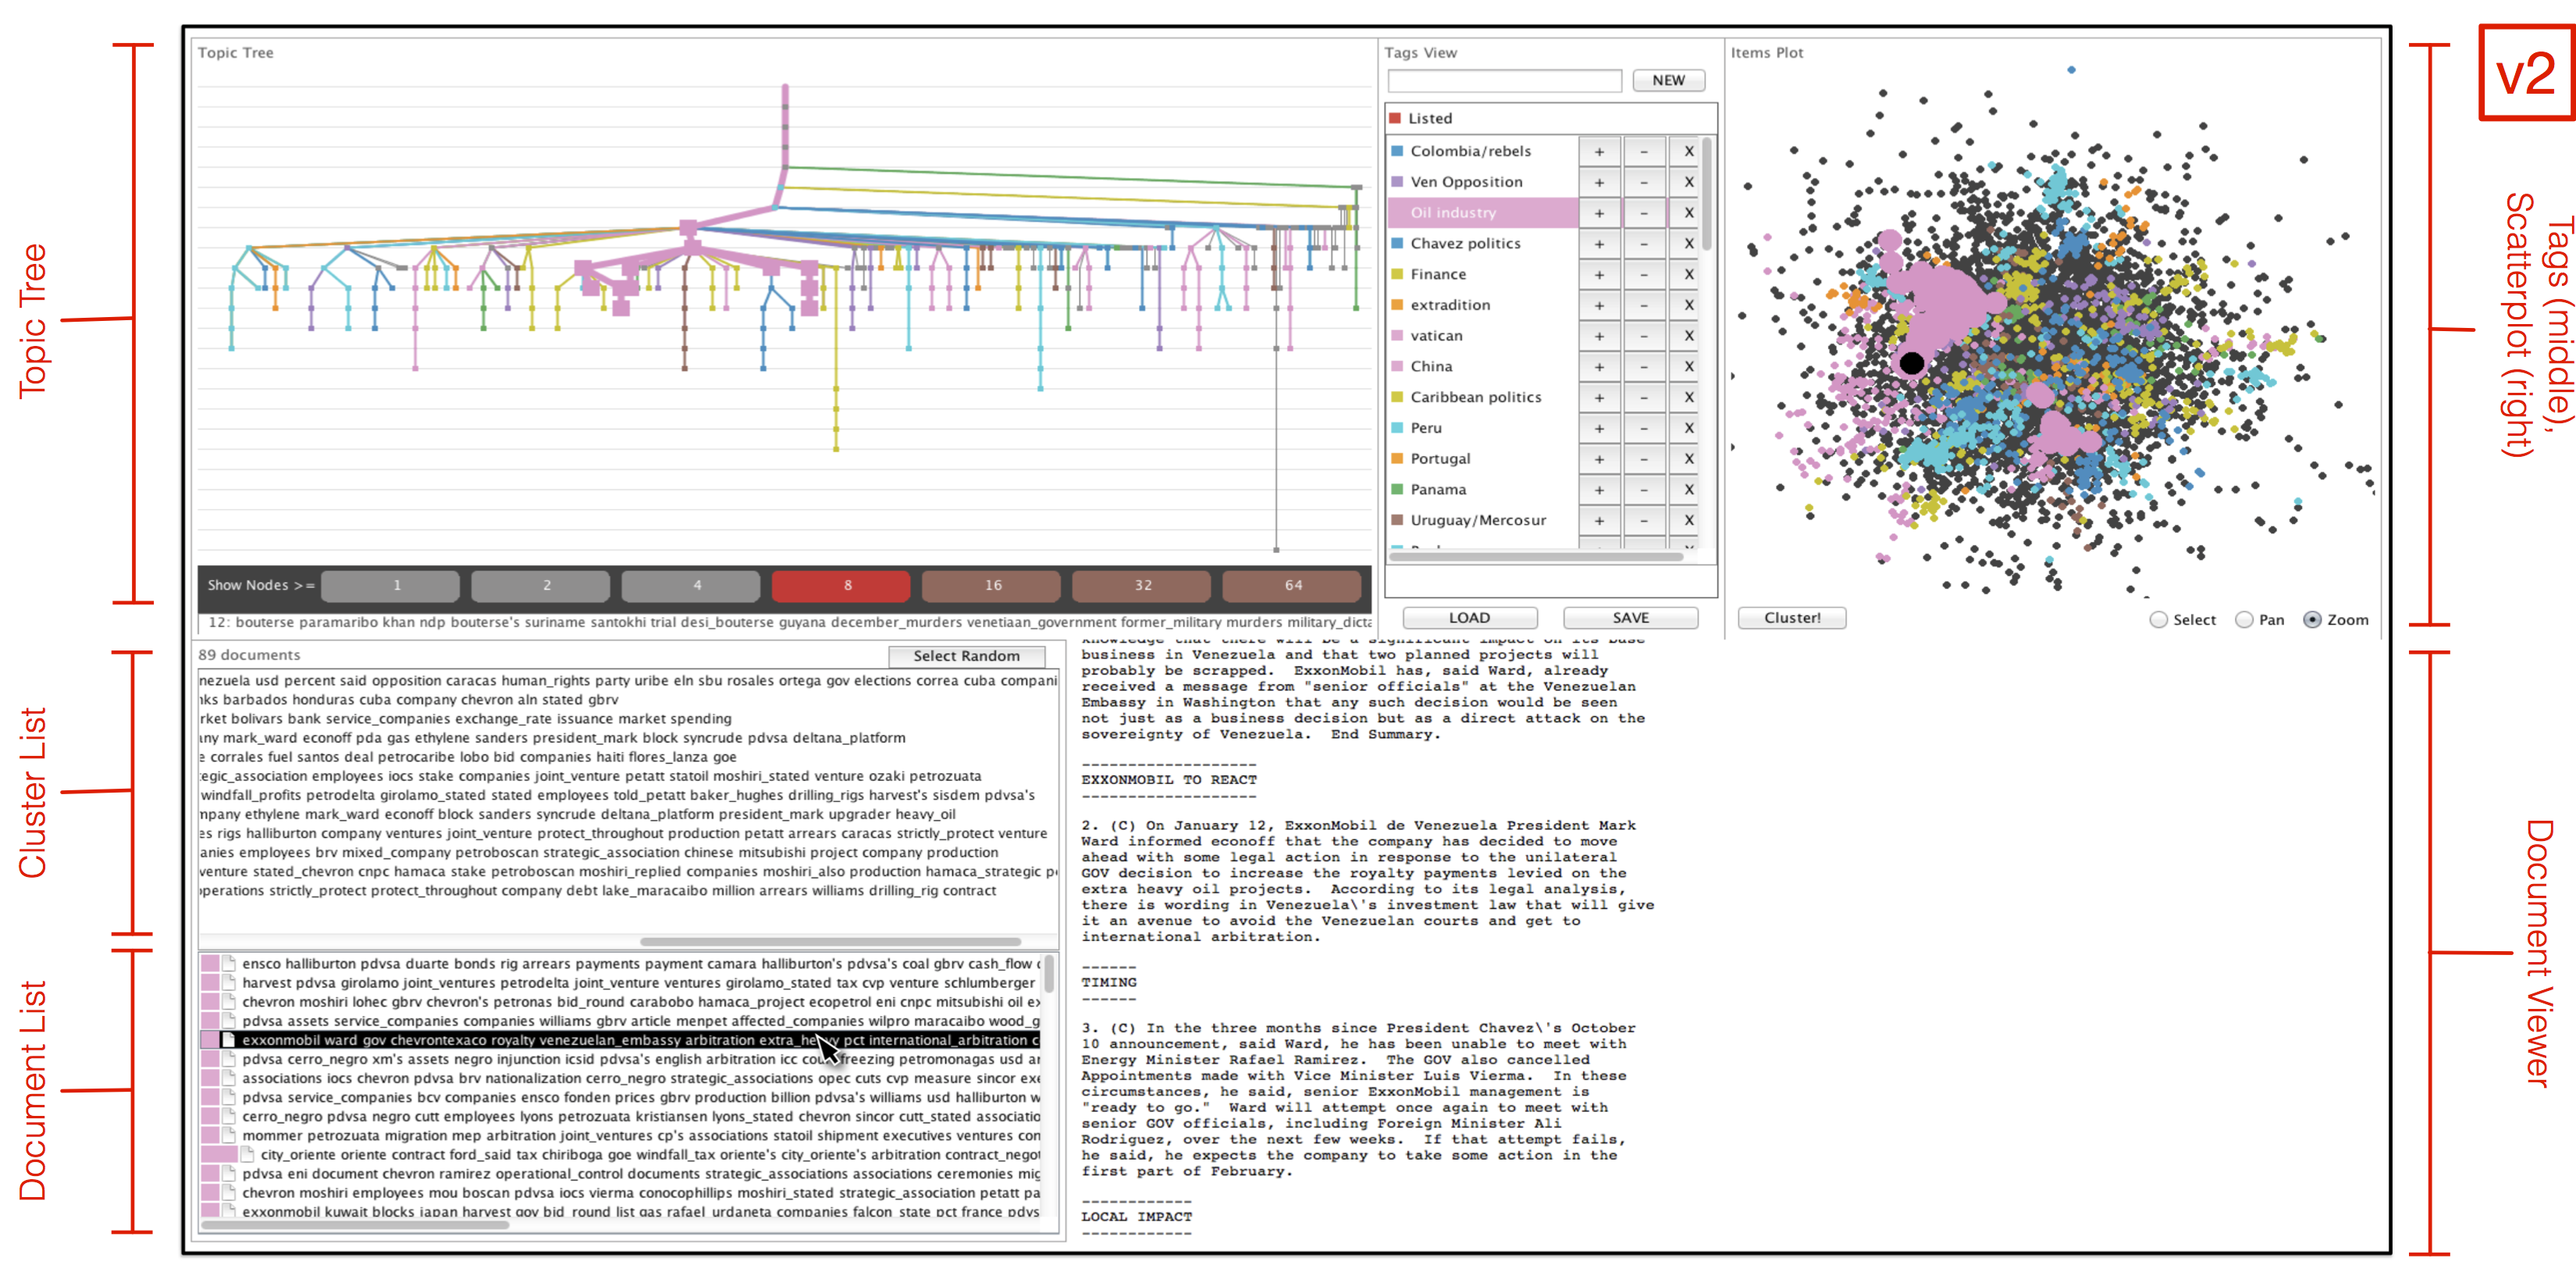
\includegraphics[width=\textwidth]{figures/overview-v2-annotated.png}
	\caption
	[
	    \textsl{Overview v2}, a desktop application released in Winter 2012.
	]
	{
    	\textsl{Overview v2}, a desktop application released in Winter 2012.
    	Shown here is 6,849 of the U.S. State Department diplomatic cables released by WikiLeaks, those pertaining to Venezuela.
    	The \textsl{``Oil industry''} tag is {\tt selected}; clusters containing documents having this tag are emphasized in pink in the \textsl{Topic Tree} and are shown in the \textsl{Cluster List} as a set of keywords.
    	Individual documents having the \textsl{``Oil industry''} tag are emphasized in the scatterplot and shown in the \textsl{Document List} as a set of keywords.
    	The fifth document is {\tt selected}; its contents are displayed in the \textsl{Document Viewer} and it is marked as a larger black dot in the scatterplot.
	}
	\centering
	\label{overview:fig:overview-v2}
\end{figure}

%-|-|-|-|-|-|-|-|-|-|-|-|-|-|-|-|-|-|-|-|-|-|-|-|-|-|-|-|-|-|-|-|-|-|-|-|-

%-|-|-|-|-|-|-|-|-|-|-|-|-|-|-|-|-|-|-|-|-|-|-|-|-|-|-|-|-|-|-|-|-|-|-|-|-

\begin{figure}
	\centering
	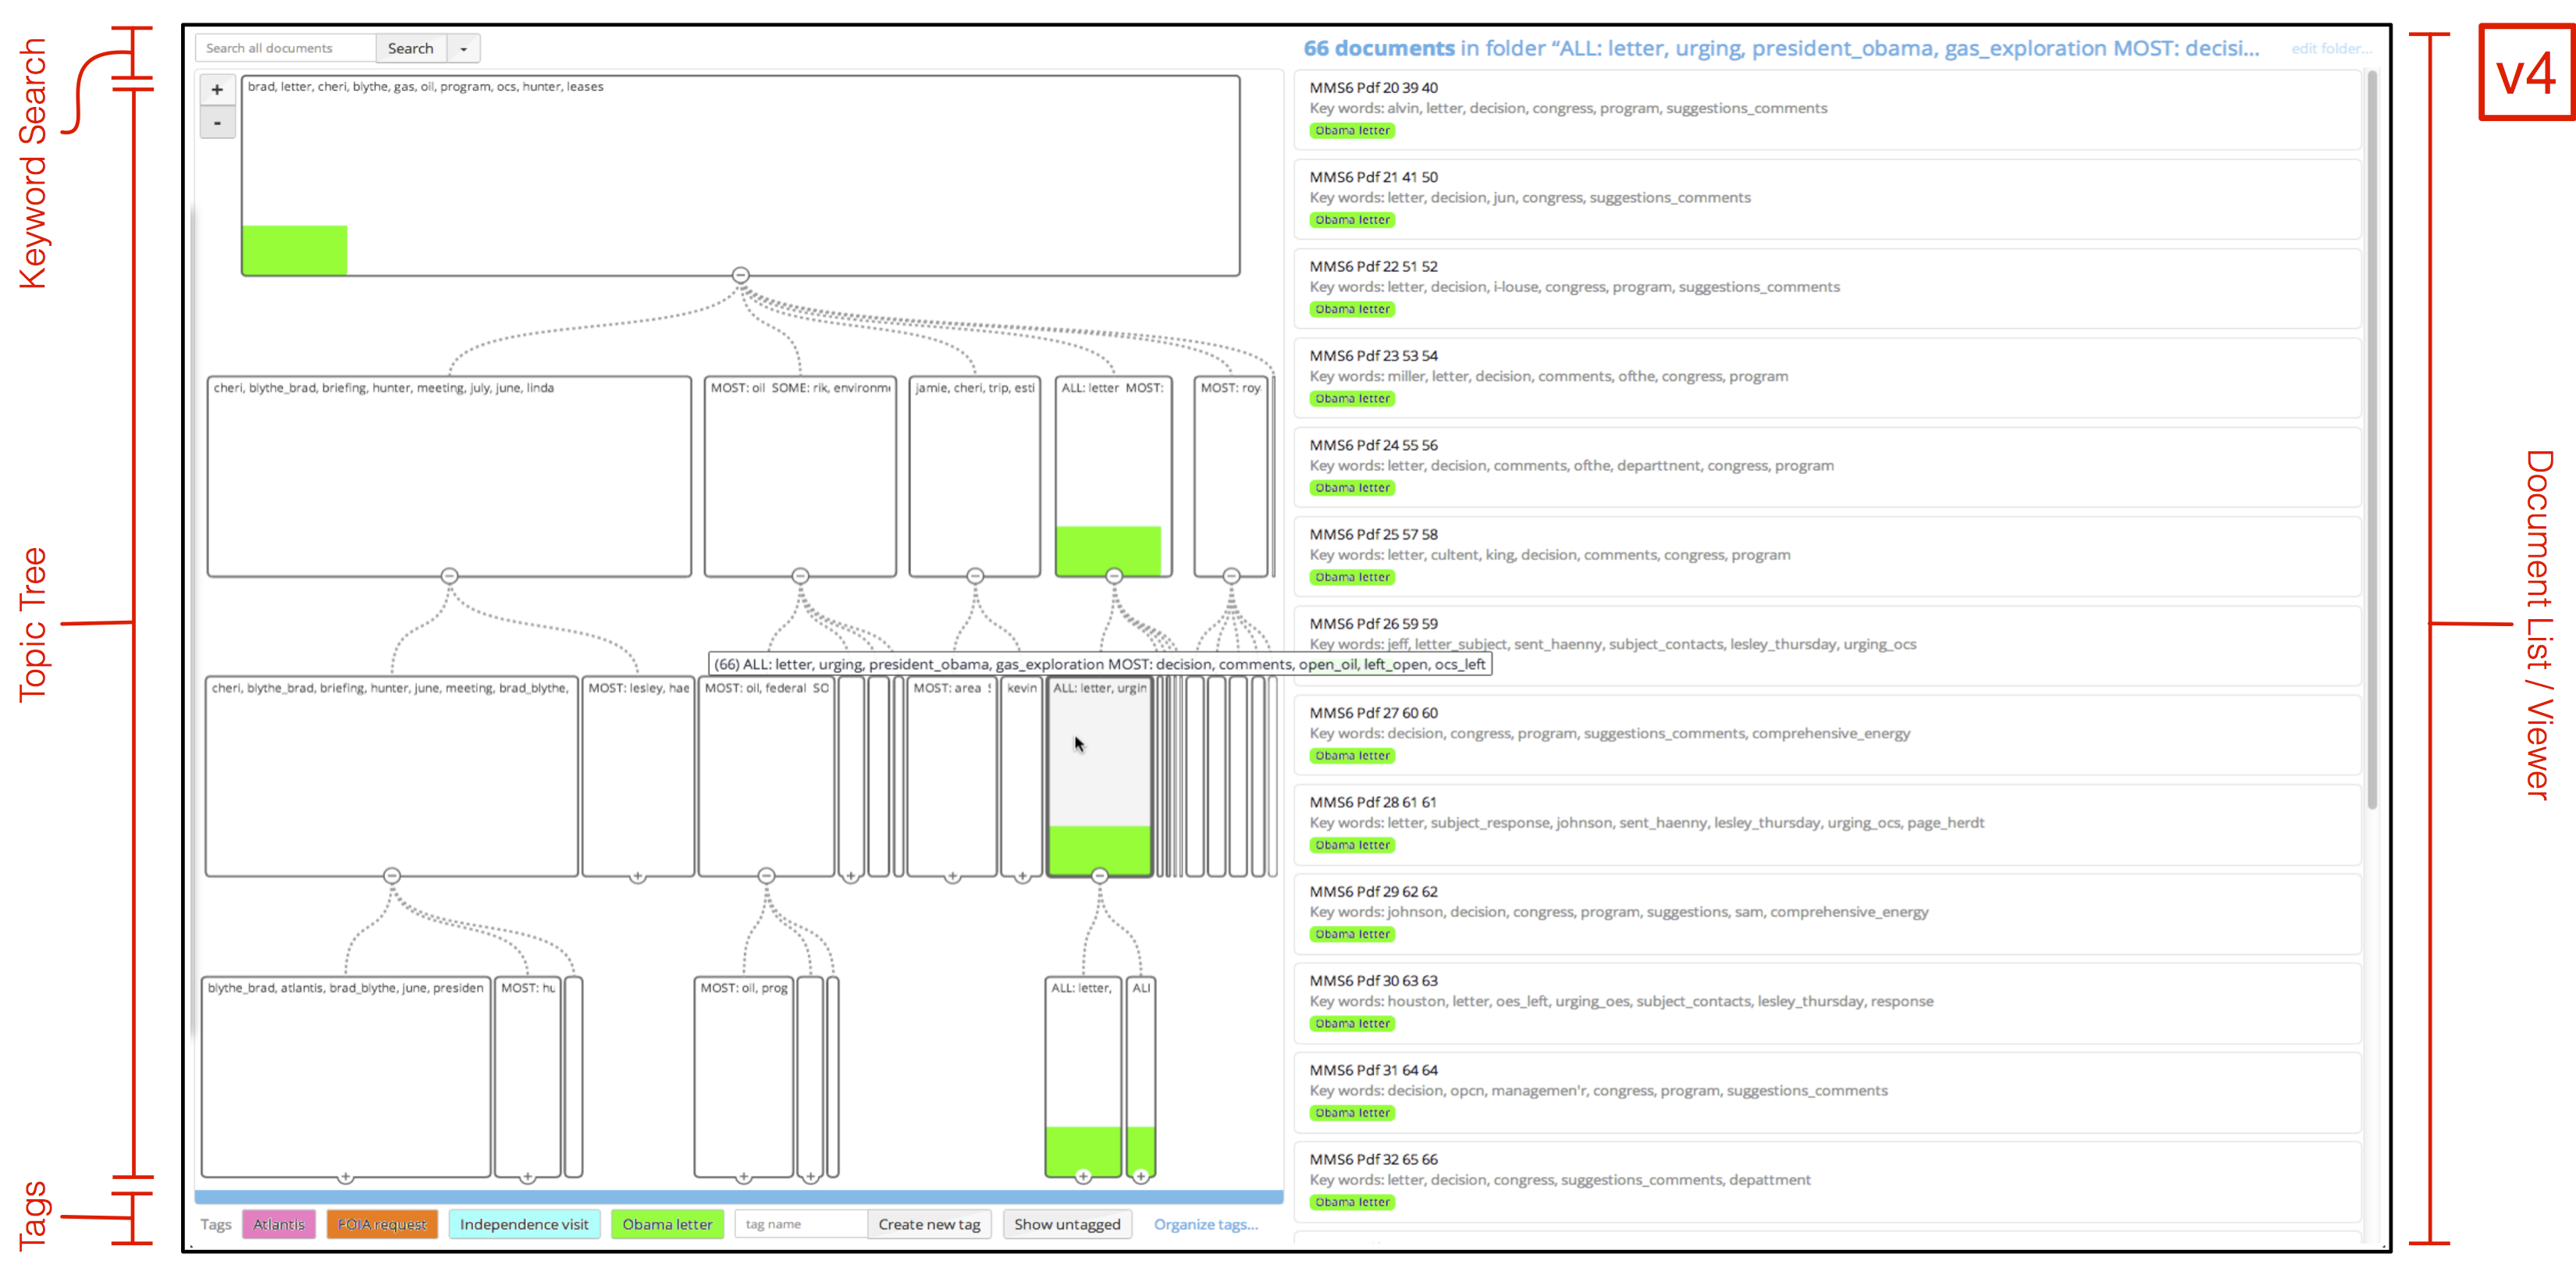
\includegraphics[width=\textwidth]{figures/overview-v4-annotated.png}
	\caption
	[
	    \textsl{Overview v4}, a web-based application released in Summer 2013.
	]
	{
    	\textsl{Overview v4}, a web-based application released in Summer 2013.
    	Shown here is 625 White House email messages concerning drilling in the Gulf of Mexico prior to the 2010 Deepwater Horizon oil spill.
    	The \textsl{``Obama letter''} tag is {\tt selected}; clusters containing documents having this tag are highlighted in green in the \textsl{Topic Tree}.
    	One of these clusters is {\tt selected} and its keywords are displayed in a tooltip; the 66 documents in this cluster are listed in the \textsl{Document List}. 
    	{\tt Selecting} a document from this list reveals the \textsl{Document Viewer} (cf. \autoref{overview:fig:overview-v4-teaser}).
	}
	\centering
	\label{overview:fig:overview-v4}
\end{figure}

%-|-|-|-|-|-|-|-|-|-|-|-|-|-|-|-|-|-|-|-|-|-|-|-|-|-|-|-|-|-|-|-|-|-|-|-|-

\bstart{Interface}
With each deployment came changes to the interface, though we will focus on the differences between {\it Overview v2} and {\it v4}, shown in \autoref{overview:fig:overview-v2} and~\ref{overview:fig:overview-v4}\footnote{A video demonstration of {\it Overview v4} is available here: \url{http://vimeo.com/71483614}.}, respectively.
The visualization design of {\it v1} and {\it v2} are quite similar to each other, as are {\it v3} and {\it v4}\footnote{Screenshots of {\it v1} and {\it v3} can be found in \autoref{app:overview} as \autoref{app:overview:fig:overview-v1} and \autoref{app:overview:fig:overview-v3}, respectively.}.  

Common to all deployed versions of {\it Overview}\index{Overview (document mining tool)} is the {\it Topic Tree}\index{visual encoding!tree} visual encoding\index{visual encoding}, representing a hierarchical clustering\index{algorithms!clustering} of similar documents\index{document data}, the {\it Document List}, showing currently {\tt selected}\index{{\tt select}} documents, the {\it Document Viewer}, and the ability to create and assign custom categorical tags to clusters or individual documents; tags are {\tt encoded}\index{{\tt encode}} as coloured labels on documents and clusters.
{\tt Selections}\index{{\tt select}} of documents are propagated and highlighted across views\index{view coordination!brushing across views}.

The {\it Topic Tree}\index{visual encoding!tree} underwent some of the most significant changes. 
It was redesigned to emphasize nodes, and to {\tt encode}\index{{\tt encode}} the number of documents in each node, instead of focusing on the edges between identically-sized nodes.
In {\it v1-v2}, the {\it Topic Tree}\index{visual encoding!tree} could be pruned based on a threshold cluster size, controlled using a set of coloured radio buttons below; in {\it v3}, we replaced threshold pruning with an open/close interface that allows a person to show or hide the children of any node.
Pan and zoom controls were also added, including an auto-zoom feature that automatically zooms and pans to a selected node.

Another prominent change was the removal of the interactive scatterplot\index{visual encoding!scatterplot}, in which individual documents were {\tt encoded}\index{{\tt encode}} by points and their placement corresponded to a two-dimensional projection of the original high-dimensional\index{high-dimensional data} \ac{TF-IDF}\index{term frequency-inverse document frequency (TF-IDF)} vector space, generated via \ac{MDS}\index{dimensionality reduction (DR)!multi-dimensional scaling (MDS)}; pairs of documents appearing closer together were deemed to be more similar than pairs of documents that were farther apart. 
The scatterplot\index{visual encoding!scatterplot} had panning and zooming controls, and document-points could be {\tt selected}\index{{\tt select}} via clicking or lassoing.

We also removed the {\it Cluster List} and consolidated the {\it Document Viewer} with the {\it Document List} (\cf \autoref{overview:fig:overview-v4-teaser}).
The {\it Document List} now displays the document title, extracted keywords, and coloured labels indicating which tags have been applied to each document.
We added full-text keyword search in {\it v4}; documents matching a search term are highlighted with colour labels in the {\it Topic Tree}\index{visual encoding!tree}, and these results can be saved as a persistent tag.
Finally, we added a {\it ``Show Untagged''} button in {\it v4}, which highlights documents and clusters where no tags have been applied, a crucial feature for the (initially unexpected) task\index{task} of exhaustively reviewing a document collection\index{document data}.

This section described the design without providing any rationale for its evolution. 
Our decisions were based on observations of real world usage; we provide concrete examples of {\it why}\index{{\tt why}} and {\it how}\index{{\tt how}} {\it Overview}\index{Overview (document mining tool)} was used by journalists\index{journalism} in \autoref{overview:usage}. 
Then, in \autoref{overview:analysis}, we present our final task abstraction\index{task!task abstraction}, the outcome of analyzing these observations, and justify our design choices with respect to these revisited tasks\index{task}. 

%-------------------------------------------------------------------------
%-------------------------------------------------------------------------

\section{Observations of Real World Usage}
\label{overview:usage}

%-------------------------------------------------------------------------
%-------------------------------------------------------------------------

We conducted six case studies\index{case study} where we analyzed the use of {\it Overview}\index{Overview (document mining tool)} by investigative journalists\index{journalism}.
We distinguish between a {\it case study}\index{case study} and a {\it usage scenario}~\cite{Sedlmair2012}\index{usage scenario}, in which the former involves a person from the target application domain who uses a tool to examine their own data, having goals related to their ongoing work; in contrast, the latter reports usage of a tool by its designers with curated data and conjectured tasks\index{task}.

\bqstart{Pilot case study}:
The first person who used {\it Overview}\index{Overview (document mining tool)} was the Associated Press Caracas bureau chief, whom we asked in November 2011 to use the {\it v1} prototype to examine 6,849 of the 251,287 U.S. State Department diplomatic cables released by WikiLeaks, those pertaining to Venezuela; this document collection\index{document data} is featured in \autoref{overview:fig:overview-v2}.
Although he found the tool to be interesting, his analysis did not lead to a published story.
This informal pilot case study\index{case study} revealed basic usability problems and the experience prompted us to formalize the case study\index{case study} process and determine foci of interest, such as utility, usability, learnability, and journalists'\index{journalism} tasks\index{task} in context.

\bstart{Metrics}
In addition to the qualitative analysis of journalists'\index{journalism} tasks\index{task}, we also focus on the metric of adoption\index{adoption} defined as {\it self-initiated} use: did a journalist\index{journalism} freely chose to use the tool for their own investigation, rather than trying out the tool in response to direct solicitation by the researchers?
According to this distinction, adoption\index{adoption} occurred in five of the six case studies\index{case study} we report, as indicated by the turquoise circles in \autoref{overview:fig:timeline}; the journalist\index{journalism} in the remaining case study\index{case study} ({\sc iraq-sec}) was co-author Stray.
We were also interested in the outcome of a journalist's\index{journalism} investigation: did they complete their investigation to satisfaction
as a result of using {\it Overview}\index{Overview (document mining tool)}, either by choosing to publish a story or by deciding that their findings did not merit a story? Or did they abandon {\it Overview}\index{Overview (document mining tool)} because the tool did not help further their investigation?

\begin{sloppypar}
\bstart{Recruitment}
Since the {\it v2} deployment, Stray has promoted {\it Overview}\index{Overview (document mining tool)} within the data journalism\index{journalism} community.
Several hundred journalists\index{journalism} have created accounts on the public server, and they have collectively uploaded more than nine million documents; {\it Overview}\index{Overview (document mining tool)} is used by approximately two hundred unique people each month\footnote{As of March 2014.}. 
As of \today, we are aware of twenty published stories where {\it Overview}\index{Overview (document mining tool)} played a part in the investigative process\footnote{Links to these stories can be found here: \url{https://github.com/overview/overview-server/wiki/News-stories}. A blog post that summarizes several of these stories is available here: \url{https://blog.overviewdocs.com/completed-stories/}}, five of which are discussed as case studies\index{case study} below.
The self-initiated journalists\index{journalism} featured in case studies\index{case study} 2--6 were recruited to participate in our study after they contacted Stray with technical questions, which often pertained to workflow\index{workflows} difficulties such as wrangling their document collection\index{document data} into a format that {\it Overview}\index{Overview (document mining tool)} could ingest.
\end{sloppypar}

\bstart{Methods}
Our case study\index{case study} findings are the result of triangulating between multiple data collection and analysis methods\footnote{\autoref{app:overview:proposal} provides additional detail regarding our data collection and analysis methodology.}.
Our primary data collection method was that of a semi-structured interview\footnote{Our interview protocol is provided in \autoref{app:overview:interview-protocol}.}.
We conducted interviews via Skype or Google$^+$ Hangout, as our journalists\index{journalism} were geographically remote; both services include a screen sharing feature, allowing journalists\index{journalism} to demonstrate aspects of their investigative process.
We recorded these interviews and demonstrations using a screen capture application and later transcribed them.
The deadline-driven nature of journalism\index{journalism} precluded multiple interviews during an ongoing investigation, so we chose to interview each journalist\index{journalism} after their investigation was complete, despite the known limitations of retrospective introspection~\cite{Ericsson1980}.
Journalists\index{journalism} were encouraged but not expected to keep a diary relating to their ongoing use of {\it Overview}\index{Overview (document mining tool)}.
Five of our case study\index{case study} journalists\index{journalism} wrote or contributed to retrospective blog posts about their process~\cite{Keller2012a,Stray2012a,Stray2012b,Stray2014,Wade2012a}, and one of them ({\sc tulsa}) also sent us his personal notes.

We also collected usage logs for each journalist\index{journalism}, consisting of timestamped interactions with {\it Overview}\index{Overview (document mining tool)}, which included {\tt selecting}\index{{\tt select}}, viewing, and {\tt annotating}\index{{\tt annotate}} documents and clusters with tags.
Log file\index{interaction!interaction logs} analysis allowed us to partially reconstruct a journalist's\index{journalism} analysis process, complementing information divulged to us in their retrospective interview.
Finally, each journalist\index{journalism} provided us with their tagged document collection\index{document data}, which helped to establish a shared context.

%-------------------------------------------------------------------------

\subsection{Case Studies}
\label{overview:case-studies}

%-------------------------------------------------------------------------


The six case studies\index{case study} we present, summarized in \autoref{overview:tab:case-studies}, took place between February 2012 and December 2013, as indicated in \autoref{overview:fig:timeline}.

\bscstart{CS1: IRAQ-SEQ~\cite{Stray2012}}
Our first case study\index{case study} took place in February 2012, when journalist\index{journalism} and co-author Stray  used {\it Overview v2} to analyze recently declassified documents from the Iraq war concerning the behavior of private security contractors.
In particular, he wanted to categorize and count types of documented incidents involving these contractors; aside from the high-profile incidents that made headlines, he wanted to determine the prevalence of other incidents that these contractors were involved in during the Iraq war.

The document collection\index{document data} was the result of a \ac{FOIA} request to the U.S. State Department, comprised of 666 incident reports over 4,500 pages, which were scanned using \ac{OCR}.
After the documents were loaded in {\it Overview}\index{Overview (document mining tool)}, Stray examined document clusters over the course of five days: he {\tt navigated}\index{{\tt navigate}} the {\it Topic Tree}\index{visual encoding!tree}, {\tt selected}\index{{\tt select}} clusters and their documents, {\tt aggregated}\index{{\tt aggregate}} clusters using the tree pruning controls, and {\tt annotated}\index{{\tt annotate}} approximately 48\% of the documents with 28 unique tags.
After a lengthy ``orientation'' phase to determine incident categories of interest, he sampled the documents using the ``Select Random'' button (above the {\it Cluster List} in \autoref{overview:fig:overview-v2}), which would {\tt select}\index{{\tt select}} a document from the {\it Document List} to be shown in the {\it Document Viewer}.
With this approach, he read and tagged 50 of the 666 reports, which allowed him to develop hypotheses regarding the prevalence of certain incident types.
Afterward, he followed up with U.S. State Department representatives, who provided additional context and a timeline for these incidents.
His published story~\cite{Stray2012} combines his categorical summarization with the context of the war.

\bscstart{CS2: TULSA~\cite{Wade2012}}
The first case of self-initiated adoption\index{adoption} by a journalist\index{journalism} took place in June 2012\footnote{Additional analysis of this case study is provided in \autoref{app:overview:proposal}.}, revealing a different motivation for using {\it Overview}\index{Overview (document mining tool)}.
In this case, the journalist\index{journalism} wanted to {\tt locate}\index{{\tt locate}} and {\tt identify}\index{{\tt identify}} evidence, documents that would support or refute a pre-existing hypothesis: he was following-up on an anonymous tip regarding municipal government mismanagement and potential conflicts of interest between city hall, municipal police, and police equipment vendors.
He filed a \ac{FOIA} request with the City Hall of Tulsa, Oklahoma for email messages between these organizations, and then used {\it Overview v2} to examine 5,996 of these email messages.

His search for corroborating evidence spanned multiple sessions over 18 days, beginning with an exhaustive and systematic left-to-right {\tt navigation}\index{{\tt navigate}} of the {\it Topic Tree}\index{visual encoding!tree}, {\tt aggregating}\index{{\tt aggregate}} clusters using the tree pruning controls, and {\tt selecting}\index{{\tt select}} clusters to view their contained documents.
He viewed roughly 70\% of the documents in the {\it Document Viewer} at least once, {\tt annotating}\index{{\tt annotate}} 92\% of them with 22 unique tags.
We observed that he undertook multiple iterations of tagging: he began by tagging entire clusters using terms appearing in cluster keywords, but later tagged individual documents throughout the tree\index{visual encoding!tree} with tags such as {\it ``important''}, {\it ``weird''}, and {\it ``follow-up.''}
As a result of this thorough tagging, the journalist\index{journalism} was able to {\tt lookup}\index{{\tt lookup}} and {\tt browse}\index{{\tt browse}} previously identified\index{{\tt identify}} clusters or documents of interest, focus on documents {\tt annotated}\index{{\tt annotate}} by multiple tags, or {\tt locate}\index{{\tt locate}} documents that remained untagged; the latter was accomplished by {\tt selecting}\index{{\tt select}} uncoloured points in the scatterplot\index{visual encoding!scatterplot}.
These tags also provided a starting point for the further {\tt annotation}\index{{\tt annotate}} of 129 {\it ``important''} documents with notes relating to his hypothesis; these notes eventually became integral parts of his published story~\cite{Wade2012}.

\bscstart{CS3: RYAN~\cite{Gillum2012}}
In October 2012, {\it Overview v2} was used yet again to {\tt locate}\index{{\tt locate}} evidence in support of a hypothesis, though there are several differences as compared to the {\sc tulsa} case study\index{case study}.
In this case, a journalist\index{journalism} wanted to follow-up on an earlier story and on accusations made by Vice President Joe Biden that vice-presidential nominee Paul Ryan's campaign statements were hypocritical.
In order to support or refute this hypothesis, the journalist\index{journalism} sought to {\tt compare} Ryan's campaign statements regarding wasteful government programs to his correspondence with various federal agencies concerning these same programs.
After filing over 200 \ac{FOIA} requests to these agencies, the journalist\index{journalism} received 8,680 pages of correspondence.
These physical documents arrived in several batches, and were scanned using \ac{OCR}.

The journalist\index{journalism} wanted to find genuine correspondence signed by Ryan; however, prevalent \ac{OCR} errors prevented him from {\tt locating}\index{{\tt locate}} these documents using keyword search. 
{\it Overview}\index{Overview (document mining tool)} was able to cluster documents effectively on the remaining intact text, and most of the documents in this collection were quickly found to be irrelevant to his hypothesis.
Over the course of half a day, he {\tt navigated}\index{{\tt navigate}} the {\it Topic Tree}\index{visual encoding!tree} to {\tt locate}\index{{\tt locate}} and {\tt identify}\index{{\tt identify}} a small subset of clusters containing one hundred and seventy-six pages of genuine correspondence containing Ryan's signature; the remainder could be safely ignored, comprised of attachments and other irrelevant correspondence.
Unlike the {\sc tulsa} journalist\index{journalism}, the {\sc ryan} journalist\index{journalism} {\tt annotated}\index{{\tt annotate}} a mere 8\% percent of the document collection\index{document data} with 12 unique tags.
As with {\sc tulsa}, the {\sc ryan} journalist\index{journalism} used tags as a starting point for the further {\tt annotation}\index{{\tt annotate}} of his source documents with notes; his published story~\cite{Gillum2012} compares these findings to Ryan's campaign statements.

\bscstart{CS4: GUNS~\cite{Keller2012}}
The first documented adoption\index{adoption} of {\it Overview}'s\index{Overview (document mining tool)} web application deployment ({\it v3}) took place in December 2012.
Shortly after the Newtown school shooting, the journalist\index{journalism} asked {\it Daily Beast} readers to self-identify as gun owners or non-owners, to report where they lived, and to post their opinion on the debate over gun ownership on a discussion board. 
He collected 1,278 comments: 757 from gun owners and 521 from non-owners.
He aimed to determine what the debate on gun ownership is about: do gun owners and non-owners raise the same issues? 
He was also curious about geographical differences.

He uploaded the responses from gun owners and non-owners into two separate instances of {\it Overview}\index{Overview (document mining tool)}.
Like the {\sc iraq-sec} case study\index{case study}, the {\sc guns} journalist\index{journalism} was interested in {\tt summarizing}\index{{\tt summarize}} a document collection\index{document data}, though the form of this {\tt summarization}\index{{\tt summarize}} was different. 
In {\sc iraq-sec}, the journalist\index{journalism} wanted to categorize and count types of documented incidents; in contrast, the {\sc guns} journalist\index{journalism} sought to {\tt identify}\index{{\tt identify}} documents that were representative of their clusters, the sensational and polarizing speaking points from both sides of the debate over gun ownership; he was less interested in a fine-grained classification or quantification.
For both sets of documents, he {\tt navigated}\index{{\tt navigate}} and {\tt selected}\index{{\tt select}} clusters and their contained documents, {\tt compared}\index{{\tt compare}} related clusters between the {\it gun owner} and {\it non-owner} instances, and later {\tt browsed}\index{{\tt browse}} previously identified clusters to {\tt identify}\index{{\tt identify}} representative quotes from people on both sides.
Ultimately, he read nearly all the discussion board comments over the course of a day.
Unlike the previous case studies\index{case study}, he did not use {\it Overview}'s\index{Overview (document mining tool)} tagging functionality, instead opting to copy quotes into an Excel\index{Excel (Microsoft)} spreadsheet, where he integrated geographical metadata and iteratively arranged\index{{\tt arrange}} quotes to construct a narrative for his story~\cite{Keller2012}.

\bscstart{CS5: DALLAS}
In August 2013, a journalist\index{journalism} used {\it Overview v4} in a similar fashion to that of the {\sc tulsa} journalist\index{journalism}, though the outcome of their investigations differed. 
In the {\sc dallas} case study\index{case study}, the journalist\index{journalism} had recently reported on a collection of 4,653 email messages resulting from a \ac{FOIA} request regarding the state government's response to an emergency incident.
The journalist\index{journalism} believed that some remaining evidence was left to be {\tt located}\index{{\tt locate}}, beyond what had already been reported in the earlier story.
Despite having already read all the documents in the collection (unassisted by {\it Overview}), the journalist\index{journalism} used {\it Overview}\index{Overview (document mining tool)} to verify that nothing was overlooked and sought to gather material for a follow-up story.
She subsequently used {\it Overview}\index{Overview (document mining tool)} to examine four additional collections of messages, analyzed individually, ranging in size between 1,858 and 3,564 email messages.

The keyword search feature introduced in {\it Overview v4} was found to be particularly useful: the journalist\index{journalism} alternated between {\tt identifying}\index{{\tt identify}} clusters by {\tt navigating}\index{{\tt navigate}}, {\tt aggregating}\index{{\tt aggregate}}, and {\tt selecting}\index{{\tt select}} nodes in the {\it Topic Tree}\index{visual encoding!tree}, and {\tt locating}\index{{\tt locate}} documents via keyword search, then {\tt identifying}\index{{\tt identify}} related documents.
As her analysis progressed, we observed that the journalist\index{journalism} relied more upon keyword search to highlight clusters of interest within the {\it Topic Tree}\index{visual encoding!tree}.
She applied tags to each of the five document collection\index{document data}s: the number of tags ranged between three and seven, and between 7\% and 52\% of documents were {\tt annotated}\index{{\tt annotate}} with at least one tag; in total, 14 out of 31 tags were created from keyword search results.

In this case, {\it Overview}\index{Overview (document mining tool)} was used to make the decision {\it not} to publish: after 12 hours of {\it Overview}\index{Overview (document mining tool)} usage spanning several weeks, the journalist\index{journalism} was sufficiently confident that nothing significant had been overlooked in the previous investigation, ultimately deciding not to write a follow-up story.
This journalist\index{journalism} estimated that it would have taken ``more than a week'' to reach this conclusion without {\it Overview}\index{Overview (document mining tool)}, and is ``definitely planning on using it again for large document sets''.

\bscstart{CS6: NY~\cite{Playford2013}}
The final case study\index{case study} we report took place in December 2013, in which a journalist\index{journalism} used {\it Overview v4} to confirm that a document collection\index{document data} {\it did not} contain evidence that would refute his hypothesis.
In the {\sc ny} case study\index{case study}, the journalist\index{journalism} had gathered material to investigate the state of New York's process for handling and responding to police misconduct cases, including 1,680 proposed and passed bills retrieved from the State Senate Open Legislation \ac{API}. 
He hypothesized that the state legislature had failed to pass any bills addressing this misconduct by increasing oversight.

A considerable amount of data wrangling was required before this journalists could use {\it Overview}\index{Overview (document mining tool)}. 
The State Senate \ac{API} provided the bills in \ac{JSON} format; to address this, the journalist\index{journalism} wrote a script to {\tt import}\index{{\tt import}} these documents into a database, which was in turn used to export a \ac{CSV} file that {\it Overview}\index{Overview (document mining tool)} could ingest. 

Following data ingestion, the journalist\index{journalism} used Overview for about four hours over the course of three days to read {\it all} the document titles and keywords in a systematic fashion: starting with the smaller nodes, he would {\tt select}\index{{\tt select}} a node in the {\it Topic Tree}\index{visual encoding!tree} and scan the document titles and keywords appearing in the {\it Document List}; the titles tended to be verbose and descriptive, and any that were deemed interesting were read in the {\it Document Viewer} or tagged as {\it ``review'' }. 
He eventually examined the largest node, which contained 732 documents with similar titles and keywords, their contents mostly comprised of boilerplate text; the journalist\index{journalism} tagged the entire node as {\it ``no unless''}, meaning that any document contained by the node was not significant unless there was another tag on it. 
He later returned to documents tagged with {\it ``review''}, replacing this tag with one of five descriptive tags.
Though the tag highlighting used in {\it Overview}'s\index{Overview (document mining tool)} {\it Topic Tree}\index{visual encoding!tree} allowed the journalist\index{journalism} to quickly {\tt locate}\index{{\tt locate}} tagged documents, he suggested that the tree\index{visual encoding!tree} could alternatively hide all documents {\it not} marked with a particular tag, such as his {\it ``not of interest''} tag.

His approach was similar to {\sc tulsa} and {\sc dallas}, in that they all sought to {\tt locate}\index{{\tt locate}} and {\tt identify}\index{{\tt identify}} clusters containing potential evidence.
However, the {\sc tulsa} and {\sc dallas} journalists\index{journalism} could have stopped their search once this evidence was found, as it is unlikely that any additional evidence would invalidate their previous findings.
In contrast, the {\sc ny} journalist\index{journalism} sought to prove the {\it non-existence} of evidence, which required review of every document, as any evidence that went overlooked would have invalidated a claim of non-existence.

As a result of his analysis, the journalist\index{journalism} was confident that no bills had been passed to address police misconduct, though several relevant bills had been proposed multiple times; conveniently, multiple versions of proposed bills were clustered together in {\it Overview}'s\index{Overview (document mining tool)} {\it Topic Tree}\index{visual encoding!tree}.
While this finding is reported in a only a single paragraph of his published story~\cite{Playford2013}, it played a key role in his argument that the state of New York is facing a police oversight problem; this story received considerable acclaim from the journalism\index{journalism} community and was a finalist for the 2014 Pulitzer Prize\footnote{\url{http://www.pulitzer.org/finalists/5325}}.

%-|-|-|-|-|-|-|-|-|-|-|-|-|-|-|-|-|-|-|-|-|-|-|-|-|-|-|-|-|-|-|-|-|-|-|-|-

\begin{table}\renewcommand{\arraystretch}{1.2}\addtolength{\tabcolsep}{-1pt}
  \begin{center}
  \tiny
  \begin{tabular}{|p{0.07\textwidth}|>{\RaggedRight}p{0.12\textwidth}|>{\RaggedRight}p{0.12\textwidth}|>{\RaggedRight}p{0.12\textwidth}|>{\RaggedRight}p{0.12\textwidth}|>{\RaggedRight}p{0.12\textwidth}|>{\RaggedRight}p{0.12\textwidth}|}

    \hline

    \cellcolor{gray!20}

    {\it {\bf Case Study}}

    & 1: {\sc iraq-sec}~\cite{Stray2012}

    & 2: {\sc tulsa}~\cite{Wade2012}

    & 3: {\sc ryan}~\cite{Gillum2012}

    & 4: {\sc guns}~\cite{Keller2012}

    & 5: {\sc dallas}

    & 6: {\sc ny}~\cite{Playford2013}

    \\

    \hline
    \cellcolor{gray!20}
    {\it Date}

	%iraq-sec
	& Feb. 2012 \raisebox{-.2\height}{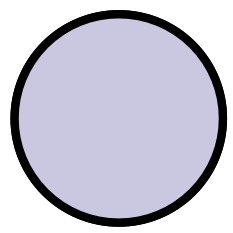
\includegraphics[width=0.015\textwidth, height=0.015\textwidth]{figures/deployment-case-study.png}}

    %Tulsa
	& Jun. 2012 \raisebox{-.2\height}{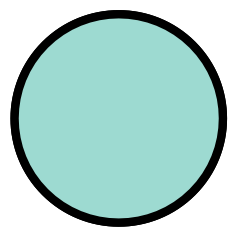
\includegraphics[width=0.015\textwidth, height=0.015\textwidth]{figures/adoption-case-study.png}}

    %Ryan
	& Oct. 2012 \raisebox{-.2\height}{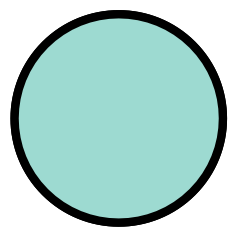
\includegraphics[width=0.015\textwidth, height=0.015\textwidth]{figures/adoption-case-study.png}}

    %Guns
	& Dec. 2012 \raisebox{-.2\height}{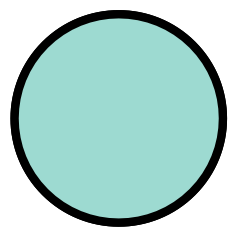
\includegraphics[width=0.015\textwidth, height=0.015\textwidth]{figures/adoption-case-study.png}}

    %Dallas
	& Aug. 2013 \raisebox{-.2\height}{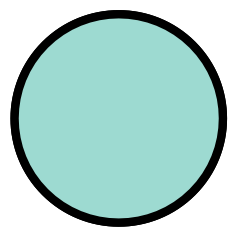
\includegraphics[width=0.015\textwidth, height=0.015\textwidth]{figures/adoption-case-study.png}}

    %NewYork
	& Dec. 2013 \raisebox{-.2\height}{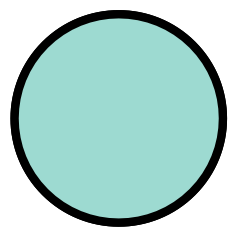
\includegraphics[width=0.015\textwidth, height=0.015\textwidth]{figures/adoption-case-study.png}}

    \\

    \cellcolor{gray!20}
    {\it Version}

	%iraq-sec
	& {\it v2} / desktop

    %Tulsa
	& {\it v2} / desktop

    %Ryan
	& {\it v2} / desktop

    %Guns
	& {\it v3} / web

    %Dallas
	& {\it v4} / web

    %NewYork
	& {\it v4} / web

    \\

    \hline
    \cellcolor{gray!20}
    {\it Document Collection}

    %iraq-sec
    &666 reports / 4,500 pages from \ac{FOIA} (scanned using \ac{OCR}).

    %Tulsa
    &5,996 email messages from \ac{FOIA}.

    %Ryan
    &8,680 pages of correspondence from multiple \ac{FOIA}s (scanned using \ac{OCR}).

    %Guns
    & 2 collections of online discussion board comments (757 in the first, 521 in the second).

    %Dallas
    & 5 collections of email messages from \ac{FOIA}s, ranging from 1,858 to 4,653 messages.

	%NewYork
    & 1,680 proposed and passed bills retrieved with NY Senate Open Legislation \ac{API}.
    
    \\

    \hline
	\cellcolor{gray!20}
    {\it Task}

    %iraq-sec
    & {\bf T1}: {\tt generate\index{{\tt discover}} hypotheses $\rightarrow$ explore\index{{\tt explore}} $\rightarrow$ summarize\index{{\tt summarize}}}

    %Tulsa
    & {\bf T2}: {\tt verify\index{{\tt discover}} hypotheses $\rightarrow$ locate\index{{\tt locate}} $\rightarrow$ identify}\index{{\tt identify}}

    %Ryan
    & {\bf T2}: {\tt verify\index{{\tt discover}} hypotheses $\rightarrow$ locate\index{{\tt locate}} $\rightarrow$ identify}\index{{\tt identify}}

    %Guns
    & {\bf T1}: {\tt generate\index{{\tt discover}} hypotheses $\rightarrow$ explore\index{{\tt explore}} $\rightarrow$ summarize\index{{\tt summarize}}}

    %Dallas
    & {\bf T2}: {\tt verify\index{{\tt discover}} hypotheses $\rightarrow$ locate\index{{\tt locate}} $\rightarrow$ identify}\index{{\tt identify}}

	%NewYork
    & {\bf T2}: {\tt verify\index{{\tt discover}} hypotheses $\rightarrow$ locate\index{{\tt locate}} $\rightarrow$ identify}\index{{\tt identify}}
    
    \\

    \hline
	\cellcolor{gray!20}
    {\it Outcome}

    %iraq-sec
    & Summarized\index{{\tt summarize}} prevalence of document categories.

    %Tulsa
    & Located\index{{\tt locate}} evidence supporting hypothesis.

    %Ryan
    & Located\index{{\tt locate}} a small subset of document clusters relevant to hypothesis.

    %Guns
    & Summarized\index{{\tt summarize}} using exemplar documents. 

    %Dallas
    & Could not locate\index{{\tt locate}} evidence to support hypothesis.

	%New York
    & Proved non-existence of evidence.
    
    \\

    \hline

  \end{tabular}
  \caption
  [
    A summary of the six case studies.
  ]
  {
    A summary of the six case studies; deployment-phase case studies are represented as \raisebox{-.2\height}{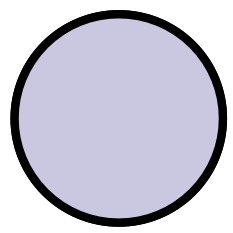
\includegraphics[width=0.015\textwidth, height=0.015\textwidth]{figures/deployment-case-study.png}} (purple circles),while adoption-phase case studies are represented as \raisebox{-.2\height}{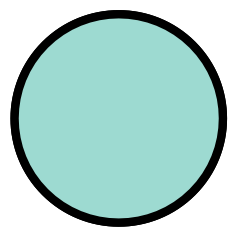
\includegraphics[width=0.015\textwidth, height=0.015\textwidth]{figures/adoption-case-study.png}} (turquoise circles).
  }
  \label{overview:tab:case-studies}
  \end{center}
\end{table}

%-|-|-|-|-|-|-|-|-|-|-|-|-|-|-|-|-|-|-|-|-|-|-|-|-|-|-|-|-|-|-|-|-|-|-|-|-

%-------------------------------------------------------------------------

\subsection{Think-Aloud Evaluation}
\label{overview:eval-usability}

%-------------------------------------------------------------------------

To complement our case study\index{case study} observations, we also solicited feedback from other journalists\index{journalism}.
After the deployment of the web-based {\it Overview}\index{Overview (document mining tool)} {\it v3}, which included usage tracking, we observed that {\it Overview}\index{Overview (document mining tool)} and its individual features were not being used to the extent that we had hoped.
We suspected usability problems so we embarked on a discount usability testing program inspired by the work of \citet{Nielsen2000}: five na\"{i}ve journalists\index{journalism} were independently presented with an example document collection\index{document data}, such as the collection featured in \autoref{overview:fig:overview-v2}, and asked to narrate their actions as they interacted with {\it Overview}\index{Overview (document mining tool)} using a think-aloud\index{evaluation!think-aloud evaluation} protocol\footnote{Think-aloud protocols are limited in that they do not capture automatic, non-conscious reactions to stimuli. The retrospective introspection of our case study\index{case study} interviews is similarly limited. Interaction logs and screen captures may provide some indication of non-conscious reactions to stimuli. Eye-tracking equipment may provide additional indication of these reactions. However, these think-aloud sessions were performed opportunistically in non-laboratory settings, and we were unable to gather additional data.}, resulting in a qualitative understanding of usability problems.
% RR: p. 86. Think-aloud protocols. Do these really capture what's going on? People's conscious understanding of why they do what they do is iffy at best. (cf. the low rate of adoption described on p. 96.) And what about the use of automatic, non-conscious procedures? Shouldn't we design for them?

All who participated in these think-aloud sessions found {\it Overview}\index{Overview (document mining tool)} to be confusing; much of this confusion was due to the visual complexity of its multiple-view interface, as well as a lack of affordances for common and critical interactions\index{interaction}, such as {\tt selecting}\index{{\tt select}} a document to read. 
We suspect that many previous document set visualization tools would face similar usability problems in real workflows\index{workflows}, either by lacking a robust document {\tt import}\index{{\tt import}} feature, or by not providing a means\index{task!means} to read individual documents~\cite{Cui2011}.
An exception is Jigsaw, whose developers have noted and overcome similar problems \cite{Gorg2014}.
In the next section, we discuss how the design of {\it v4} resolved these usability problems.

%-------------------------------------------------------------------------
%-------------------------------------------------------------------------

\section{Analysis}
\label{overview:analysis}

%-------------------------------------------------------------------------
%-------------------------------------------------------------------------

Given our observations or real world usage, we now revisit our initial task abstraction\index{task!task abstraction} and discuss the rationale for {\it Overview}'s\index{Overview (document mining tool)} design.

%-------------------------------------------------------------------------

\subsection{Task Abstractions Reconsidered}
\label{overview:task-abstraction-reconsidered}

%-------------------------------------------------------------------------

% \js{
% iraq-sec -> summarize by classification
% tulsa -> locate evidence
% gun -> summarize through exemplars
% ryan -> locate subset
% dallas -> locate evidence
% newyork -> prove non-existence
% }

After the {\sc guns} case study\index{case study}, we struggled to distinguish between journalists'\index{journalism} goals, approaches, and outcomes.
Specifically, the {\sc tulsa} and {\sc ryan} journalists\index{journalism} used {\it Overview}\index{Overview (document mining tool)} in more directed and systematic ways that we did not anticipate, in that they sought to {\tt locate}\index{{\tt locate}} specific evidence or a subset of clusters that were relevant to a pre-existing hypothesis, forcing us to reconsider our initial task abstraction\index{task!task abstraction} of {\it ``exploring''}\index{{\tt explore}} a document cluster structure, which was based on the {\sc warlogs} use case.
A number of previous tools aim to help people to {\it ``explore''}\index{{\tt explore}} a document collection\index{document data} (\eg~\cite{Chaney2012,Cui2011,Dou2013,Endert2012b}), though few of these tools have been evaluated\index{evaluation} with people who work in a specific target domain who bring their own data, making us suspect that this imprecise term often masks a lack of understanding of the tasks\index{task} that people perform.

In48 \autoref{ch:typology}, we proposed a typology\index{task!task typology} of abstract visualization tasks\index{task!task abstraction}, the purpose of which was precisely to articulate such differences in the use of visualization tools at multiple levels of abstraction. 
According to this typology\index{task!task typology}, a task\index{task} description is broken down into {\it why}\index{{\tt why}} data is visualized, {\it what}\index{{\tt what}} dependencies a task\index{task} might have, and {\it how}\index{{\tt how}} the task\index{task} is supported.
{\it How}\index{{\tt how}} is somewhat orthogonal to {\it why}\index{{\tt why}}, as exemplified by the differences in usage reported in the previous section.
We applied this typology\index{task!task typology} to the coding\index{coding (qualitative data analysis)} of our observational data, characterizing two different tasks\index{task}, {\bf T1} and {\bf T2}, that replace and improve upon our initial task abstraction\index{task!task abstraction}. 
In this section, we will use the vocabulary and notation of this typology\index{task!task typology} to focus on {\it why}\index{{\tt why}} and {\it what}\index{{\tt what}}; in \autoref{overview:rationale}, we analyze {\it how}\index{{\tt how}} {\it Overview}\index{Overview (document mining tool)} supports these tasks\index{task}.

\bstart{T1: {\tt generate hypotheses} $\rightarrow$ {\tt explore} $\rightarrow$ {\tt summarize}}
When approaching a collection of leaked documents or a corpus of social media content, a journalist\index{journalism} may have little prior knowledge regarding the collection's content, eliciting a need to {\tt generate hypotheses}\index{{\tt discover}} and to ask {\it ``what's in this collection?''}.
To support the generation of hypotheses, a journalist\index{journalism} must be able to {\tt explore}\index{{\tt explore}} a document collection\index{document data} and {\tt summarize}\index{{\tt summarize}} clusters of documents.
The term {\tt explore}\index{{\tt explore}} is defined more precisely in our typology\index{task!task typology} as a form of {\tt search}\index{{\tt search}} in which neither the identity nor the location of a search target are known a priori.
In the context of a document collection\index{document data}, a search target may be content within a document, an individual document itself, a cluster of related documents, or an arbitrary set of documents and clusters.
{\tt Exploring}\index{{\tt explore}} is distinguished from {\tt browsing}\index{{\tt browse}}, in which the location of a search target is known but its identity is not, {\tt locating}\index{{\tt locate}}, in which the converse is true, and {\tt lookup}\index{{\tt lookup}}, in which both the location of the target and its identity are known. 
The result of {\tt summarizing}\index{{\tt summarize}} is a compressed representation of the full contents of the document collection\index{document data}, such as the categories and counts produced in the {\sc iraq-sec} case study\index{case study}, or the exemplar documents that the journalist\index{journalism} ultimately {\tt selected}\index{{\tt select}} in {\sc guns} case study\index{case study}.

\bstart{T2: {\tt verify hypotheses} $\rightarrow$ {\tt locate} $\rightarrow$ {\tt identify}}
In contrast, a journalist\index{journalism} who asks for documents via \ac{FOIA} request typically has some pre-existing hypotheses, and their aim is to {\tt verify}\index{{\tt discover}}, {\tt refute}, or {\tt refine} these hypotheses by {\tt locating}\index{{\tt locate}} evidence.
In these cases, a journalist\index{journalism} likely has a sense of what the documents are about, but they may not be able to specify the evidence they seek in terms of a standard keyword search (for example, ``corruption'' would not suffice), and there may also be unexpected but valuable material waiting to be discovered.
In the language of our typology\index{task!task typology}, the aim is to {\tt locate}\index{{\tt locate}} and {\tt identify}\index{{\tt identify}} clusters containing potential evidence, beginning with those labelled by interesting keyword terms; alternatively, a journalist\index{journalism} will {\tt locate}\index{{\tt locate}} documents containing specific search terms and subsequently {\tt browse}\index{{\tt browse}} and {\tt identify}\index{{\tt identify}} related documents found in the same cluster.
{\bf T2} describes the use of {\it Overview}\index{Overview (document mining tool)} in the {\sc tulsa}, {\sc ryan}, {\sc dallas}, and {\sc ny} case studies\index{case study}.

Throughout both {\bf T1} and {\bf T2}, a journalist\index{journalism} will often {\tt produce}\index{{\tt produce}} notes or annotations\index{{\tt annotate}} for documents as they {\tt generate}\index{{\tt discover}}, {\tt verify}\index{{\tt discover}}, or {\tt refine} their hypotheses, perhaps {\tt comparing}\index{{\tt compare}} documents to each other or to secondary sources outside of the collection.
{\bf T1} and {\bf T2}, along with the subsequent annotation task, are illustrated using the visual notation of our typology\index{task!task typology} in \autoref{fig:overview:tasks} and \autoref{fig:overview:tasks:annotate}, respectively, in the addendum (\autoref{overview:addendum}) at the end of this chapter.

%-------------------------------------------------------------------------

\subsection{Design Rationale}
\label{overview:rationale}

%-------------------------------------------------------------------------

With a more precise understanding of journalists'\index{journalism} tasks\index{task}, we now analyze the rationale for our visual encoding\index{visual encoding} and interaction\index{interaction} design choices in the hope that our choices may transfer to other domain problems involving similar data\index{data abstraction} and task abstractions\index{task!task abstraction}.

\bqstart{Why show a tree?}
{\it Trees\index{visual encoding!tree} afford structured and systematic exploration\index{{\tt explore}}.}
When a document collection\index{document data} contains separable clusters of similar documents, a tree-based visual encoding\index{visual encoding!tree} affords a systematic and, if desired, exhaustive traversal of these clusters. 
The {\sc tulsa} case study\index{case study} is an example where the journalist\index{journalism} based his choice of which documents to read based on the structure of the tree\index{visual encoding!tree}, sweeping from left to right.
The {\it Topic Tree}\index{visual encoding!tree} also includes a visual encoding\index{visual encoding} of applied tags, which makes it possible for a person to {\tt identify}\index{{\tt identify}} the documents they have and have not already tagged, and how tags correspond to clusters.

\bqstart{How to show a tree?}
{\it Emphasize interior nodes (not edges or leaves); instill trust\index{trust} in the underlying algorithm.}
The {\it Topic Tree}\index{visual encoding!tree} in the first two versions of {\it Overview}\index{Overview (document mining tool)} (\autoref{overview:fig:overview-v2}) rendered all clusters as identical nodes.
While tree-based visual encodings\index{visual encoding!tree} are often associated with the task\index{task} of path tracing and determining connectivity~\cite{Lee2006}, people who use {\it Overview}\index{Overview (document mining tool)} are primarily interested in the properties of nodes corresponding to document clusters, such as the number of documents contained by a cluster, or the key terms that describe these documents.

The {\it Topic Tree}\index{visual encoding!tree} of {\it v3-4} directly {\tt encodes}\index{{\tt encode}} cluster size as node width; this design choice allows a person to {\tt compare}\index{{\tt compare}} cluster sizes directly, or work systematically from larger to smaller topics, of particular use when trying to {\tt summarize}\index{{\tt summarize}} a document collection\index{document data} to some desired degree of detail ({\bf T1}).
In enlarging the width of nodes, it also became possible to {\tt encode}\index{{\tt encode}} the number of documents tagged within the cluster as a colour label having a width proportional to the size of the node, as shown in \autoref{overview:fig:overview-v4}.
We opted not to use a space-filling treemap\index{visual encoding!treemap} visual encoding\index{visual encoding} of hierarchical document clusters\index{document data} because this approach would place too much emphasis on leaf nodes; when {\tt summarizing}\index{{\tt summarize}} a collection ({\bf T1}) or when {\tt locating}\index{{\tt locate}} a subset of documents ({\bf T2}), the mid-level interior nodes in the tree\index{visual encoding!tree} are typically the most informative.
While less space efficient, a tree\index{visual encoding!tree} with variable-width nodes provides more flexibility, especially given the differences between {\bf T1} and {\bf T2}.

With larger nodes, we were able to display cluster keyword terms directly in the node itself, rather than in a separate {\it Cluster List} view, as in {\it v1-2}, which displayed keywords only for the selected\index{{\tt select}} cluster and its descendants.
Displaying keywords within nodes allows a person to {\tt compare}\index{{\tt compare}} keywords at a glance, both between and within clusters.

The design of the {\it Topic Tree}\index{visual encoding!tree} required a balance between usability and cluster fidelity: in {\it v3}, there was no limit on the number of children allowed for each node, a situation reported to be overwhelming by journalists\index{journalism} who participated in the think-aloud evaluation\index{evaluation!think-aloud evaluation}.
When a node can have many children, tree\index{visual encoding!tree} exploration\index{{\tt explore}} reduces to linear search; for this reason, the maximum number of child nodes was limited in {\it v4} by switching to a recursive adaptive {\it K}-means algorithm~\cite{Pham2005}\index{algorithms!clustering} with an upper limit of five children per node.

We added explicit cluster fidelity labels to the {\it Topic Tree}\index{visual encoding!tree} nodes in {\it v4}
to help people interpret the content of a cluster: the labels {\it ``Some''}, {\it ``Most''}, and {\it ``All''} show how many documents in a cluster contain each keyword and thus signal the consistency of topics found in that node, as shown in \autoref{overview:fig:overview-v4}.
These labels help a person to decide whether to treat the node as a conceptual unit that might be tagged as a whole, or expand it to examine its children individually.
They help a person assess cluster consistency and separability and serve to build trust\index{trust} in the clustering algorithm~\cite{Chuang2012}\index{algorithms!clustering}.
Previously, people had to judge the topical consistency of a cluster by examining the individual documents within it, or by referring to the scatterplot\index{visual encoding!scatterplot} in a way that \citet{Sedlmair2013} demonstrated to be difficult for dimensionally reduced\index{dimensionality reduction (DR)} data.

\begin{sloppypar}
\bqstart{How to interact with a tree?}
{\it Selective pruning and informative tooltips.}
In {\it v1-v2}, people were able to clarify the {\it Topic Tree}\index{visual encoding!tree} by pruning ({\tt aggregating}\index{{\tt aggregate}}) small nodes, according to a threshold {\tt selected}\index{{\tt select}} from a set of seven coloured radio buttons below the {\it Topic Tree}\index{visual encoding!tree}.
Our case studies\index{case study} revealed that many people never understood that the variable tree-pruning threshold used in {\it v1-v2} was hiding nodes from them, a problem especially for those intent on {\tt locating}\index{{\tt locate}} evidence or proving the non-existence of evidence ({\bf T2}).
We replaced threshold-based node pruning with a selective expand/collapse option on each node; when combined with panning and zooming, these interactions\index{interaction} provide people with a fine-grained control over focus and context.
\end{sloppypar}

Upon {\tt selecting}\index{{\tt select}} a node in {\it v1-v2}, keywords for the selected\index{{\tt select}} cluster and its descendants were shown in a status bar between the {\it Topic Tree}\index{visual encoding!tree} and the {\it Cluster List}, however these were spatially removed from a person's point of focus.
To resolve this, we added tooltips in {\it v3} that show cluster keywords when the cursor hovers over a node.

\bqstart{Why no scatterplot?}
{\it Unstructured exploration\index{{\tt explore}} is redundant for} {\bf T1} {\it and} {\bf T2}.
Using scatterplots\index{visual encoding!scatterplot} to visualize document collections\index{document data} is an approach common to previous work~\cite{Chen2009,Granitzer2004,Endert2012b,Leaksplorer,Paulovich2007}.
We thought that a scatterplot\index{visual encoding!scatterplot} would allow people to judge cluster size, quality, and separability~\cite{Sedlmair2013}.
However, scatterplots\index{visual encoding!scatterplot} do not directly show cluster content, such as document keywords, unless tooltips or point aggregation is used.
We did not pursue the use of these design choices because we discovered that the scatterplot\index{visual encoding!scatterplot} was seldom used in the case studies\index{case study} of journalists\index{journalism} who adopted\index{adoption} {\it Overview}\index{Overview (document mining tool)}.
The {\sc tulsa} journalist\index{journalism} was an exception in that he used the scatterplot\index{visual encoding!scatterplot} to {\tt locate}\index{{\tt locate}} untagged documents containing potential evidence after extensive use of the {\it Topic Tree}\index{visual encoding!tree} ({\bf T2}).
This task\index{task} would have been better served by providing a direct way to show how many untagged documents a node contains; the {\it ``Show Untagged''} button introduced in {\it v4} accomplishes this.

Ultimately, we realized that a scatterplot\index{visual encoding!scatterplot} does not help people overcome the burden of choice overabundance when determining which cluster to investigate next~\cite{Schwartz2003}, whereas the tree-based hierarchical clustering\index{algorithms!clustering} used in the {\it Topic Tree}\index{visual encoding!tree} affords a form of structured {\tt navigation}\index{{\tt navigate}}.
In addition, the cluster fidelity labels introduced in {\it v4} help people to assess cluster consistency and separability, thereby eliminating any further need for a scatterplot\index{visual encoding!scatterplot}.  

\bqstart{Why tags?}
{\it Tags provide simple annotation\index{{\tt annotate}}, progress tracking, and human-defined semantics.}
Tagging was used extensively in five of the six case studies\index{case study}. 
Some tags aligned with cluster boundaries ({\sc iraq-sec}, {\sc ryan}, and the first set of tags created in {\sc tulsa}), while other tags appeared throughout the tree\index{visual encoding!tree} ({\sc dallas}, {\sc ny}, and the second set of tags created in {\sc tulsa}).
Tags are a simple and flexible form of {\tt annotation}\index{{\tt annotate}} that help people track where they have been and what they have learned. 
They can also be used to impose a context-specific organization scheme on a document collection\index{document data}.
No single clustering will meet all analysis needs, since any high-dimensional dataset\index{high-dimensional data} is likely to have multiple cross-cutting semantically interesting clusterings~\cite{Grimmer2011}. 
The ``best'' clustering will depend on the documents and the story.
{\it Overview}\index{Overview (document mining tool)} does not support manual re-arrangement\index{{\tt arrange}} of the {\it TopicTree} hierarchy, as in tools such as HierarchicalTopics~\cite{Dou2013}.
Instead, we support manual tagging as a simple and flexible way for people to impose their own semantics on a document collection\index{document data}, where the cluster structure can be leveraged as a useful scaffold when it matches a person's mental model, but ignored when it does not.
The most recent feature added to {\it Overview}\index{Overview (document mining tool)}, developed after the case studies\index{case study} in this chapter, supports the creation of multiple trees\index{visual encoding!tree}, giving different views of same document collection\index{document data}. 
A person can control the clustering by entering words to ignore, which prevents {\it Overview}\index{Overview (document mining tool)} from clustering based on document letterhead or boilerplate text, and by entering especially important words which are weighted higher when constructing document vectors. 
It is also possible to create a tree\index{visual encoding!tree} containing only a subset of the documents, specified by {\tt selecting}\index{{\tt select}} an existing tag.

\bqstart{Multiple views: how many and how to coordinate?}
{\it Less is more; provide obvious affordances.}
The evolving design of {\it Overview}\index{Overview (document mining tool)} recalls the challenges and considerations for designing multiple view tools, which we have discussed elsewhere~\cite{Lam2010}.
These considerations include determining the appropriate number of discrete views, the arrangement\index{{\tt arrange}} of these views, and how these views should be coordinated\index{view coordination}.
A consensus on these questions has not yet been reached, as multiple-view visualization tools range from dual-view to over twenty, with a similar range in view coordination patterns~\cite{Weaver2007}.

The {\sc caracas} pilot case study\index{case study} with {\it Overview v1} revealed that the {\it Document Viewer} was too small and the {\tt selection}\index{{\tt select}} of documents and clusters across the different views was poorly coordinated\index{view coordination}\index{view coordination}.
Despite improvements to view coordination in {\it v2} and {\it v3}, the views were not always well understood; for example, those who participated in the think-aloud evaluation\index{evaluation!think-aloud evaluation} did not initially realize that the {\it Document List}, displayed as a line of keywords for each document, was in fact a list of {\tt selectable}\index{{\tt select}} documents.
In {\it v4}, {\it Overview}'s\index{Overview (document mining tool)} interface was streamlined into three views coordinated\index{view coordination} with linked {\tt selection}\index{{\tt select}} and highlighting: the {\it Topic Tree}\index{visual encoding!tree}, a consolidated {\it Document Viewer/List} featuring document titles and list {\tt navigation}\index{{\tt navigate}} controls, and a list of {\it Tags}; as described above, we removed the scatterplot\index{visual encoding!scatterplot} and {\it Cluster List}, both made redundant by the redesigned {\it Topic Tree}\index{visual encoding!tree}.
While we might have made {\it Overview}\index{Overview (document mining tool)} a single-view tool, we instead reasoned that having the {\it Topic Tree}\index{visual encoding!tree} visible provides helpful context when reading a document and deciding what to read next.

\bqstart{How to support workflows?}
{\it Simplify for infrequent use; reduce data wrangling.}
Our findings show that simplicity and learnability are critical for journalists\index{journalism}, because any one journalist\index{journalism} only deals with large document collections\index{document data} intermittently.

After {\it Overview v2} was deployed and promoted within the journalism\index{journalism} community, it became clear that many people had great difficulty downloading, installing, and configuring it.
Additionally, {\it v2} could only {\tt import}\index{{\tt import}} documents in a \ac{CSV} file; we quickly learned that journalists\index{journalism} receive document collections\index{document data} in every conceivable format, from stacks of paper to database dumps.
We confirmed that the need to wrangle data into compatible formats is a considerable barrier to adopting\index{adoption} a visualization tool into an analysis workflow\index{workflows}, as discussed in a recent research agenda~\cite{Kandel2011}.
We should not expect journalists\index{journalism} to write custom data wrangling scripts, as the {\sc ny} journalist\index{journalism} had to do.
To minimize the amount of configuration and wrangling required, the web-based {\it Overview v3-v4} required no installation and supported {\tt import}\index{{\tt import}} from a folder of \ac{PDF} documents or from DocumentCloud\footnote{\url{http://documentcloud.org/}}, a document hosting service used by journalists\index{journalism} which can itself ingest a wide variety of formats.
Without this integration, we suspect that the {\sc dallas} journalist\index{journalism} would have been unable to make use of {\it Overview}\index{Overview (document mining tool)}.
The DocumentCloud interface is integrated into {\it Overview}'s\index{Overview (document mining tool)} {\it Document Viewer}, which includes a function for {\tt annotating}\index{{\tt annotate}} documents with notes. 

We also added full-text keyword search in {\it v4}, as members of the journalism\index{journalism} community and our case study\index{case study} journalists\index{journalism} had expressed a desire to flexibly alternate between {\tt locating}\index{{\tt locate}} clusters in the {\it Topic Tree}\index{visual encoding!tree} and a directed search for {\tt locating}\index{{\tt locate}} documents of interest, without having to use a search tool such as grep or DocumentCloud's search interface. 
We expect that the {\sc tulsa} and {\sc ryan} journalists\index{journalism}, both performing {\bf T2} with {\it v2}, would have benefited from this keyword search feature, and that the absence of this feature would have been a deterrent for the {\sc dallas} and {\sc ny} journalists\index{journalism}, who also performed {\bf T2}.

We note that the use of {\it Overview}\index{Overview (document mining tool)} forms part of a larger investigation and reporting workflow\index{workflows}: each case study\index{case study} journalist\index{journalism} combined its use with many computer-assisted and non-computer-assisted methods for data collection, data transformation, and eventual story presentation\index{storytelling}.

\bstart{Summary}
This section presented seven lessons or guidelines that can be applied to the design of visualization tools for document data\index{document data} in particular, though we expect that these lessons may also be transferable to tools that address other forms of hierarchically-structured data\index{hierarchical data}:

\begin{itemize}
    \item Why show a tree?\index{visual encoding!tree} {\it Trees afford structured and systematic exploration\index{{\tt explore}}.}
    \item How to show a tree?\index{visual encoding!tree} {\it Emphasize interior nodes (not edges or leaves); instill trust\index{trust} in the underlying algorithm.}
    \begin{sloppypar}
    \item How to interact with a tree?\index{visual encoding!tree} {\it Selective pruning and informative tooltips.}
    \end{sloppypar}
    \item Why no scatterplot?\index{visual encoding!scatterplot} {\it Unstructured exploration\index{{\tt explore}} is redundant.}
    \item Why tags? {\it Tags provide simple annotation\index{{\tt annotate}}, progress tracking, and human-defined semantics.}
    \item Multiple views: how many and how to coordinate? {\it Less is more; provide obvious affordances.}
    \item How to support workflows?\index{workflows} {\it Simplify for infrequent use; reduce data wrangling.}
\end{itemize}

%-------------------------------------------------------------------------
%-------------------------------------------------------------------------

\section{Discussion}
\label{overview:discussion}

%-------------------------------------------------------------------------
%-------------------------------------------------------------------------

In this section, we discuss the value and logistics of conducting field studies involving multiple deployments and the analysis of adoption\index{adoption}, as well as the limitations of this type of research.

\bqstart{Why study adoption?}
As with any iterative human-centred design process, it is difficult to know when to declare success; we consider adoption\index{adoption} defined as repeated instances of self-initiated use to be a form of success. 
Adoption\index{adoption} is particularly interesting in the domain of journalism\index{journalism} because tool use is a decision made separately by each journalist\index{journalism} for each story, rather than dictated by a central authority.

Though the visualization design process is cyclical and may include multiple deployments, there are surprisingly few papers that comment on the adoption\index{adoption} of a visualization tool without the prompting of designers: in a recent survey of eight hundred visualization papers containing an evaluation\index{evaluation} component, only five commented on adoption~\cite{Lam2012}\index{adoption}. 
Of these, two provide a thorough description of who adopted\index{adoption} their visualization tool, how it had been used, whether it was still in use, and what problems people reported~\cite{Kincaid2005,McKeon2009}.
Our work adds to this short list, as does the recent study of Jigsaw's adoption~\cite{Kang2012}\index{adoption}.

Many visualization design studies\index{design studies} report on deployment to a target group of individuals and evaluate\index{evaluation} their reaction to the tools during a period of intense study, but our own experience and personal communication with other practitioners leads us to believe that visualization tool use typically drops off after a paper is submitted. 
\citet{Gonzalez2003a} provide a rare example of explicitly checking back after this time period; they found that their target population did not adopt\index{adoption} the visualization tool despite the promising initial results reported in their original paper, and conjecture that a misunderstanding of workflow\index{workflows} was the primary factor behind this lack of adoption\index{adoption}. 
We conjecture that this situation might be the common case, and that longer-term adoption\index{adoption} rates may be very low for research prototypes. 
Sustained follow-up by researchers until adoption\index{adoption} is achieved provides a way to disambiguate whether the barrier to adoption\index{adoption} is truly only a workflow\index{workflows} issue, or an indication that the tool failed to address the true needs of the people for whom the tool was built.

\bstart{The logistics of studying adoption}
Before {\it Overview}\index{Overview (document mining tool)} was deployed, we could not have fully predicted {\it why}\index{{\tt why}} and {\it how}\index{{\tt how}} journalists\index{journalism} would approach large document collections\index{document data}; we were unable to verify the correctness of our task\index{task!task abstraction} and data abstractions\index{data abstraction}.
{\it Overview}\index{Overview (document mining tool)} is sufficiently novel that its value could not be assessed without adequately functional prototypes.
We argue that this situation is common in visualization because of the complexity of the data and tasks\index{task} at play, recalling the argument of \citet{Lloyd2011} about the need for {\it data sketches}\index{data sketch}: functional example designs for establishing context of use and eliciting requirements\footnote{Unlike typical \ac{HCI} approaches such as paper prototyping, functional example designs in a visualization context entails the development of interactive software prototypes.}.
They contrasted their design-first approach, illustrated by the red trajectories in \autoref{overview:fig:hcd-loops}, to a design-then-evaluate\index{evaluation} approach (the green trajectory) and to an approach grounded in a person's context~\cite{Isenberg2008} (the blue trajectory).
The purple trajectory illustrates that close collaboration with domain experts from the very start of a project means they bring expertise about requirements to the table, so it is not a design-first endeavour. 
The multiple loops in the purple trajectory emphasize the importance of deploying a visualization tool as a precursor to evaluation\index{evaluation}, and we note that after these loops the trajectory ends at context of use: it took several deployments and case studies\index{case study} of self-initiated journalists\index{journalism} who adopted\index{adoption} {\it Overview}\index{Overview (document mining tool)} before we attained a clear understanding of journalists'\index{journalism} tasks\index{task} and their broader analysis workflows\index{workflows}.

%-|-|-|-|-|-|-|-|-|-|-|-|-|-|-|-|-|-|-|-|-|-|-|-|-|-|-|-|-|-|-|-|-|-|-|-|-

 \begin{figure}
	\centering
	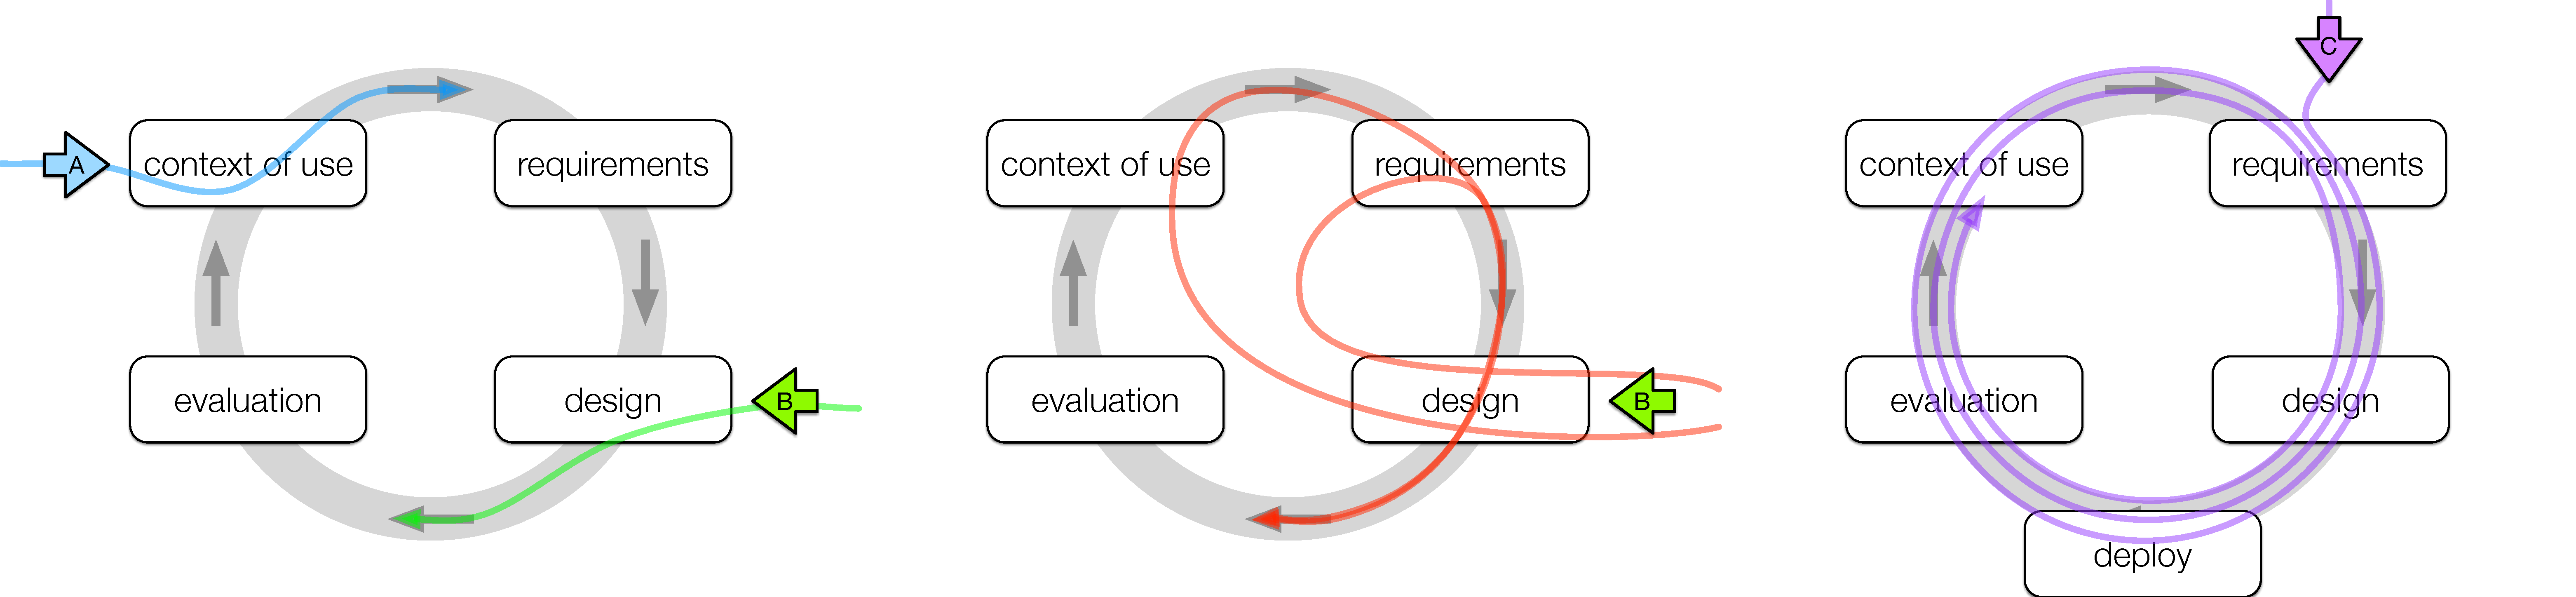
\includegraphics[width=\textwidth]{figures/hcd-loops}
	\caption
	[
	    The human-centred design process development cycle.
	]
	{
	    The human-centred design process development cycle, in which \citet{Lloyd2011} discern between alternative entry points (A,B) and between design-then-evaluate (green), grounded (blue), and their own approach in which example designs are used to establish context of use and elicit requirements (red). In contrast, we begin with some requirements at point C, and only after multiple deployments do we arrive at a clear understanding of context of use (purple). Figure adapted and extended from \citet{Lloyd2011}.
	}
	\centering
	\label{overview:fig:hcd-loops}
\end{figure}

%-|-|-|-|-|-|-|-|-|-|-|-|-|-|-|-|-|-|-|-|-|-|-|-|-|-|-|-|-|-|-|-|-|-|-|-|-

Our use of case studies\index{case study} to study adoption\index{adoption} is methodologically similar to qualitative longitudinal evaluation\index{evaluation} studies described in previous work~\cite{Lloyd2011,Saraiya2006,Shneiderman2006}.
Our approach differs from these in that we engaged a different set of people at each stage of design, rather than the same set of people.
This difference reflects {\it Overview}'s\index{Overview (document mining tool)} context of use: repeat usage cannot be predicted and {\it Overview}\index{Overview (document mining tool)} is only appropriate for some investigations; we have yet to encounter a journalist\index{journalism} who specializes in investigations pertaining to large document collections\index{document data}.

%-------------------------------------------------------------------------
%-------------------------------------------------------------------------

\section{Summary}
\label{overview:conclusion}

We presented a field study of {\it Overview}\index{Overview (document mining tool)}, an application for the systematic analysis of large document collections\index{document data}.
{\it Overview}\index{Overview (document mining tool)} has proven to be useful, having been used in investigations leading to at least nine published stories.
Using the typology\index{task!task typology} of visualization tasks proposed in \autoref{ch:typology}, we characterized two task abstractions\index{task!task abstraction} based on findings from six case studies\index{case study}.
Given our data and task abstractions\index{task!task abstraction}, we rigorously analyzed the effectiveness of {\it Overview}'s\index{Overview (document mining tool)} visual encoding\index{visual encoding} and interaction\index{interaction} design.
Our analysis may transfer beyond the domain of journalism\index{journalism}, and speaks to the design and evaluation\index{evaluation} of other visualization tools for supporting the analysis of document collections\index{document data} and clustered dimensionally reduced\index{dimensionality reduction (DR)} data.
Finally, this work adds to the small number of studies found in the visualization literature that include observations of adoption\footnote{While studies of adoption and appropriation may be common in the \ac{HCI} community, they are rare in the visualization literature.}\index{adoption}; in observing real world usage by self-initiated journalists\index{journalism}, we presented detailed evidence to support the contention that that several iterations of design and deployment are required before fully understanding {\it why}\index{{\tt why}} and {\it how}\index{{\tt how}} a visualization tool will be used in practice.

%-------------------------------------------------------------------------
%-------------------------------------------------------------------------

\section{Addendum}
\label{overview:addendum}

\autoref{fig:overview:tasks}\footnote{\autoref{fig:overview:tasks} and \autoref{fig:overview:tasks:annotate} did not appear in our paper about {\it Overview}~\cite{Brehmer2014}.} illustrates the two tasks\index{task} that we characterized in \autoref{overview:task-abstraction-reconsidered}; colours correspond to the {\it why-what-how} structure of our task typology\index{task!task typology} (see \autoref{typology:fig:typology})\footnote{We use the revised typology described in \autoref{drvistasks:typology}.}.
\autoref{fig:overview:tasks} indicates the {\it how}\index{{\tt how}} and {\it what}\index{{\tt what}} aspects of these two tasks\index{task} explicitly, as this information was discussed implicitly throughout this chapter. 
In {\bf T1}, the {\tt input}\index{{\tt input}} is a document collection\index{document data} and the {\tt output}\index{{\tt output}} is evidence to either refute or verify\index{{\tt discover}} a hypothesis.
In {\bf T2}, the {\tt input}\index{{\tt input}} is once again a document collection\index{document data}, however the {\tt output}\index{{\tt output}} is a set of exemplar documents or a set of clusters that can be used to {\tt summarize}\index{{\tt summarize}} the entire collection.
{\it Overview}\index{Overview (document mining tool)} supports both of these tasks\index{task} via {\tt encoding}\index{{\tt encode}} the document collection\index{document data} as a tree\index{visual encoding!tree}, by allowing people to interactively {\tt navigate}\index{{\tt navigate}} this tree structure\index{visual encoding!tree}, to {\tt select}\index{{\tt select}} clusters and individual documents, to {\tt aggregate}\index{{\tt aggregate}} (or disaggregate) clusters of documents using the interactive expand and collapse controls on each node of the tree\index{visual encoding!tree}.

\autoref{fig:overview:tasks:annotate} depicts a task\index{task} that follows either {\bf T1} or {\bf T2}, in which the person who uses {\it Overview}\index{Overview (document mining tool)} will {\tt annotate}\index{{\tt annotate}} clusters or individual documents with meaningful tags (a {\tt produce}\index{{\tt produce}} action)\footnote{As per the discussion in \autoref{drvistasks:typology}, we now view {\tt annotate} as a form of {\tt produce}, as indicated in \autoref{fig:overview:tasks:annotate}.}.
To {\tt annotate}\index{{\tt annotate}} documents or clusters with tags, a person {\tt selects}\index{{\tt select}} documents or clusters, {\tt selects}\index{{\tt select}} a tag, and the tag is {\tt encoded}\index{{\tt encode}} as a coloured label for the document or cluster.

%-|-|-|-|-|-|-|-|-|-|-|-|-|-|-|-|-|-|-|-|-|-|-|-|-|-|-|-|-|-|-|-|-|-|-|-|-

 \begin{figure}
	\centering
	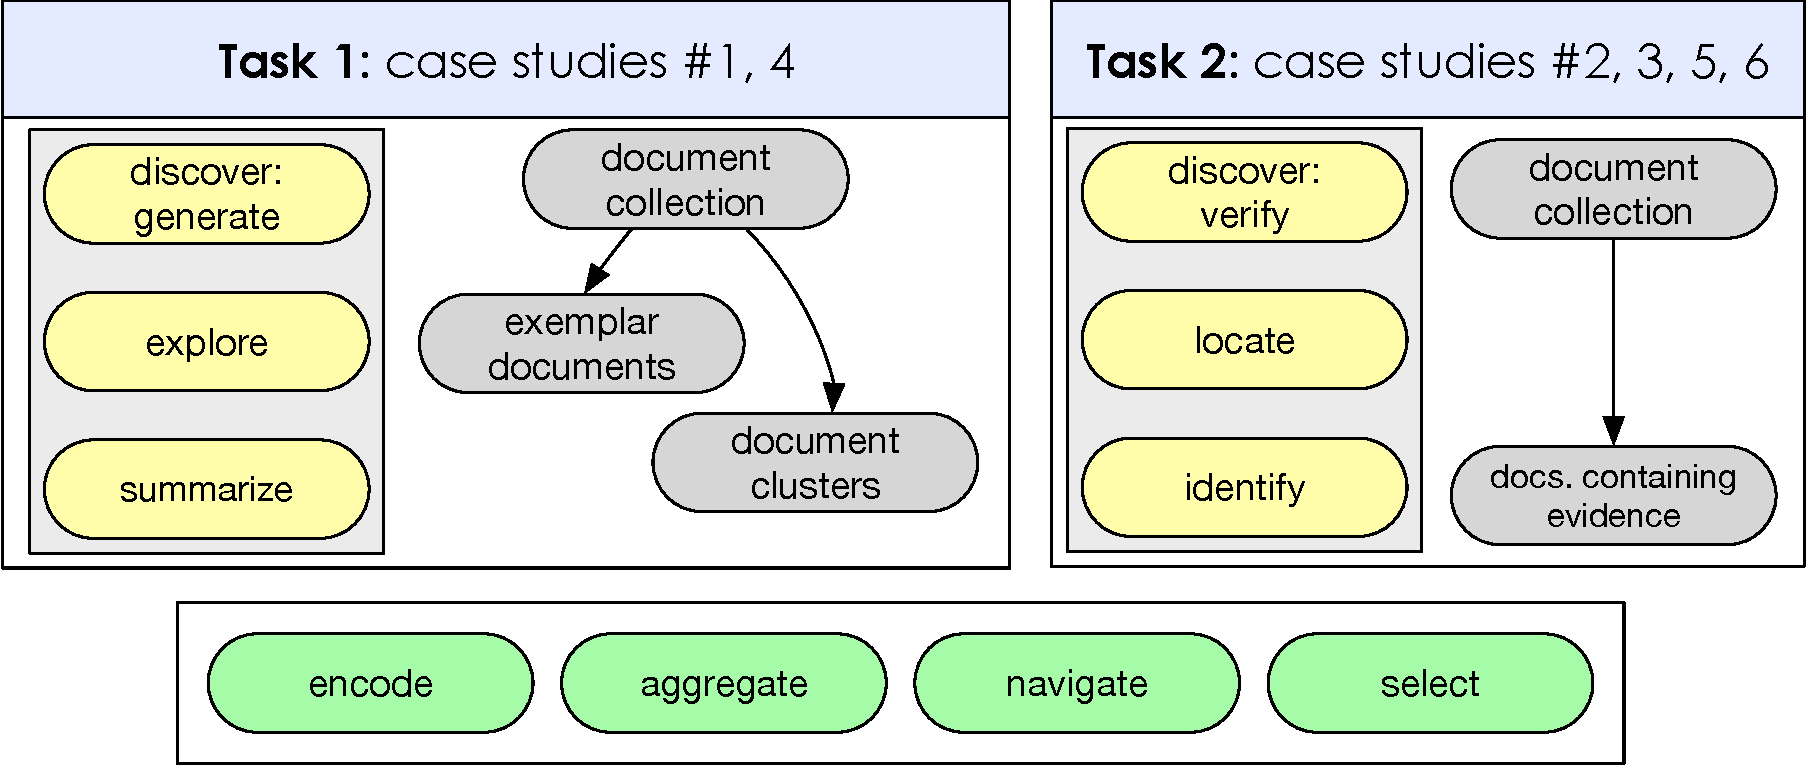
\includegraphics[width=\textwidth]{figures/overview-tasks}
	\caption
	[
	   The two tasks characterized in \autoref{overview:task-abstraction-reconsidered}.
	]
	{
	   The two tasks characterized in \autoref{overview:task-abstraction-reconsidered}; colours correspond to the {\it why-what-how} structure of our task typology (see \autoref{typology:fig:typology}), where yellow is {\it why}, green is {\it how}, and grey is {\it what} defined in terms of {\tt inputs} and {\tt outputs}.
	}
	\centering
	\label{fig:overview:tasks}
\end{figure}

%-|-|-|-|-|-|-|-|-|-|-|-|-|-|-|-|-|-|-|-|-|-|-|-|-|-|-|-|-|-|-|-|-|-|-|-|-

%-|-|-|-|-|-|-|-|-|-|-|-|-|-|-|-|-|-|-|-|-|-|-|-|-|-|-|-|-|-|-|-|-|-|-|-|-

 \begin{figure}
	\centering
	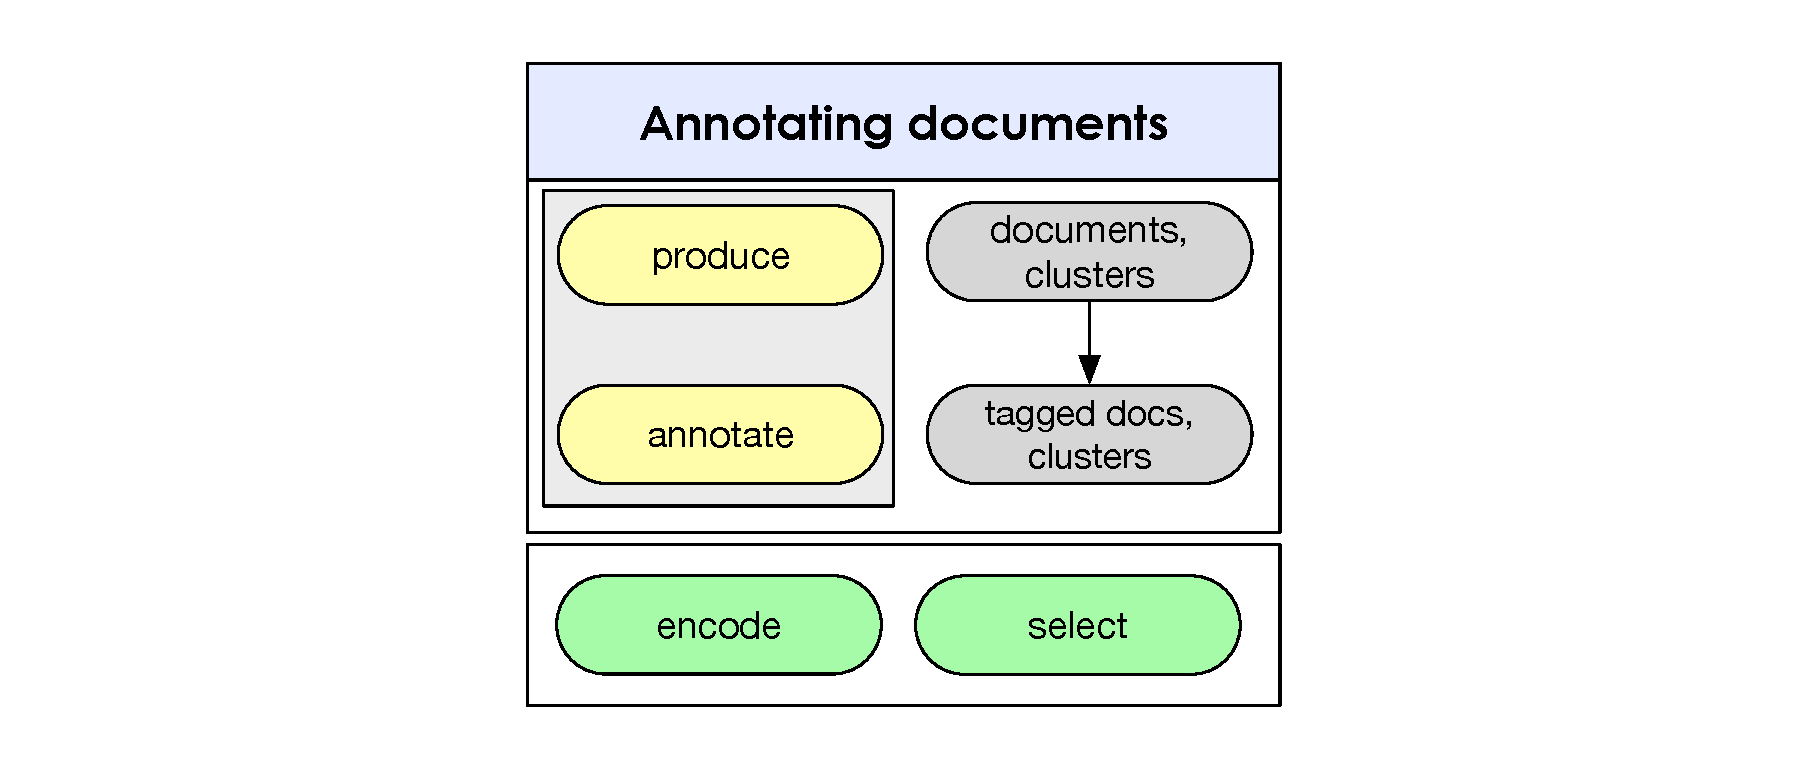
\includegraphics[width=\textwidth]{figures/overview-tasks-2}
	\caption
	[
	    The task of {\tt annotating} documents and clusters.
	]
	{
	   The task of {\tt annotating} documents and clusters (which follows {\bf T1} or {\bf T2}); colour conventions follow that of \autoref{fig:overview:tasks}.
	}
	\centering
	\label{fig:overview:tasks:annotate}
\end{figure}

%-|-|-|-|-|-|-|-|-|-|-|-|-|-|-|-|-|-|-|-|-|-|-|-|-|-|-|-|-|-|-|-|-|-|-|-|-

\endinput
